\documentclass{crm-article}

\usepackage{graphicx}
\usepackage{amsmath} 
\usepackage{bm}
\usepackage{amsbsy} 
\usepackage{amssymb}
\usepackage{cite}
\usepackage{multirow}

\graphicspath{{./eps/}}


\begin{document}

%\englishpaper % раскомментировать в том случае, если текст статьи на английском языке

%\norussian % раскомментировать, если нет метаданных на русском

%\affiliationnoref % раскомментировать, если автор один или все авторы из одной организации

%\emailnoref % раскомментировать в том случае, если автор единственный

%\year=2021 % current year by default
%\journalVol{10}
%\journalNo{1} %выпуска
\setcounter{page}{1}

% раздел журнала
\journalSection{Математические основы и численные методы моделирования}
\journalSectionEn{Mathematical modeling and numerical simulation}


% дата получения
%\journalReceived{01.02.2021.}
%\journalReviewed{01.02.2021.}
%принято к публикации
%\journalAccepted{01.02.2021.}


\UDC{519.63}
\title{Численное моделирование нестационарных задач переноса нейтронов в SP$_3$ приближении}
\titleeng{Numerical modeling of non-stationary problems of neutron transport in the SP$_3$ approximation}
\thanks{Работа выполнена при поддержке гранта Российского Научного Фонда \#19-71-00008}%если имеется
\thankseng{This work was supported by the grant of the Russian Science Foundation \#19-71-00008}

%автор - в формате \author{\firstname{И.\,И.}~\surname{Иванов}}
\author{\firstname{Александр.\,В.}~\surname{Аввакумов}}
%автор - в формате \authorfull{Имя Отчество Фамилия}
\authorfull{Александр Владимирович Аввакумов}
% автор на англ. - в формате \authoreng{\firstname{I.\,I.}~\surname{Ivanov}}
\authoreng{\firstname{A.\,V.}~\surname{Avvakumov}}
%автор на англ. - в формате \authorfull{Firstname M. Surname}
\authorfulleng{Aleksandr V. Avvakumov}
%вписать свою электронную почту
\email{avvakumov2009@rambler.ru}
%организация - в формате \affiliation{Московский государственный университет,\protect\\ Россия, 141700, г. Москва, ул. Университетская, д. 9}
\affiliation{Национальный исследовательский центр <<Курчатовский институт>>,\protect\\ Россия, 123182, г. Москва, пл. Академика Курчатова, д. 1}
%организация - в формате \affiliationeng{Moscow State Institute University, 9 University street, Moscow, 141700, Russia}
\affiliationeng{National Research Center <<Kurchatov Institute>>,\protect\\ 1, Akademika Kurchatova pl., Moscow, 123182, Russia}

% повторите блок для каждого автора;
% если авторов несколько, и автоматическая расстановка сносок от фамилий 
% к организациям приводит к неправильным результатам, укажите правильный 
% вариант в квадраных скобках

\author[2]{\firstname{Петр\,Н.}~\surname{Вабищевич}}
\authorfull{Петр Николаевич Вабищевич}
\authoreng{\firstname{P.\,N.}~\surname{Vabishchevich}}
\authorfulleng{P.\,N. Vabishchevich}
\email{vabishchevich@gmail.com}
\affiliation[2]{Институт проблем безопасного развития атомной энергетики РАН,\protect\\ Россия, 115191, г. Москва, ул. Большая Тульская, д. 52}
\affiliationeng{Nuclear Safety Institute of Russian Academy of Science,\protect\\ 52, Bolshaya Tulskaya Street, Moscow, 115191, Russia}

\author[3]{\firstname{Александр\,О.}~\surname{Васильев}}
\authorfull{Александр Олегович Васильев}
\authoreng{\firstname{A.\,O.}~\surname{Vasilev}}
\authorfulleng{A.\,O. Vasilev}
\email{haska87@gmail.com}
\affiliation[3]{Северо-Восточный федеральный университет им. М.К. Аммосова,\protect\\ Россия, 677000, г. Якутск, ул. Белинского, д. 58}
\affiliationeng{North-Eastern Federal University,\protect\\ 58, Belinskogo Street, Yakutsk, 677000, Russia}

\author[2]{\firstname{Валерий\,Ф.}~\surname{Стрижов}}
\authorfull{Валерий Федорович Стрижов}
\authoreng{\firstname{V.\,F.}~\surname{Strizhov}}
\authorfulleng{V.\,F. Strizhov}
\email{vfs@ibrae.ac.ru}


\begin{abstract}
Моделирование динамических процессов в ядерных реакторах осуществляется чаще всего на основе уравнения переноса нейтронов в многогрупповом диффузионном приближении.
Использование диффузионного приближения позволяет проводить полномасштабные расчеты активной зоны с высоким быстродействием и приемлемой точностью. Однако, для ряда вычислений точность диффузионного приближения оказывается недостаточной.
Транспортное SP$_3$ приближение уравнения переноса нейтронов позволяет повысить точность расчетов по сравнению с диффузионным приближением.
Кроме того, вычислительные затраты SP$_3$ расчетов намного меньше, чем у других транспортных методов более высокого порядка (таких как S$_N$ или P$_N$).
Еще одним преимуществом SP$_3$ приближения является аналогичная структура уравнений, которая используется в диффузионном приближении.
Следовательно, не составит особого труда реализовать вариант решения с использованием SP$_3$ приближения для многогрупповых диффузионных кодов, которые преимущественно применяются для практических расчетов.
В связи с этим, будет очень полезно сравнить результаты рассчитанные как диффузионным, так и транспортным SP$_3$ методами.

В данной работе рассматривается SP$_3$ приближение для нестационарной задачи многогруппового переноса нейтронов.
Применение SP$_3$ методологии основано на решении $\lambda$-спектральной задачи. 
Динамические процессы протестированы на примере двугруппового бенчмарка реактора TWIGL-2D.
Для достижения геометрической общности применяется метод конечных элементов.
Контроль точности решения проводился на последовательности сгущающихся сеток с использованием конечных элементов различной степени.
Результаты рассчитанные диффузионным и транспортным SP$_3$ методами сравниваются с результатами эталонных расчетов. 
\end{abstract}

\keyword{уравнение переноса нейтронов}
\keyword{$\lambda$-спектральная задача}
\keyword{диффузионное приближение}
\keyword{SP$_3$ приближение}
\keyword{twigl}

\begin{abstracteng}
Modeling of dynamic processes in nuclear reactors is carried out, mainly, on the basis of the multigroup diffusion approximation for the neutron flux.
The diffusion approximation allows full-scale whole-core calculations with high speed and reasonable accuracy. However for some caculations, the diffusion approximation accuracy is unsufficient. 
The SP$_3$ approximation of the neutron transport equation allows improving the calculational accuracy compared with the diffusion approximation. 
Besides, the SP$_3$ calculation are less expensive than high-order transport methods (such as S$_N$ or P$_N$). 
Another advantage of the SP$_3$ approximation is a similar structure of equations as in the diffusion method. 
Therefore, it is easy to implement the SP$_3$ solution option to the multi-group neutron diffusion codes, which are mainly used for practical calculations. 
In this regard, it will be very useful to compare the results, calculated by both the diffusion and transport SP$_3$ methods.

In this paper we consider the SP$_3$ approximation for the steady-state multigroup neutron transport problem.
Application of the SP$_3$ methodology is based on solution of the $\lambda$-spectral problem. 
Dynamic behaviour has been tested for the twogroup TWIGL-2D reactor benchmark test. 
The finite element method is chosen to achieve the geometrical generality. 
The control of the solution accuracy was carried out on a sequence of refining grids using finite elements of varying degrees.
The results calculated with the diffusion and SP$_3$ methods are compared with the reference calculation results. 
\end{abstracteng}

\keywordeng{neutron transport equation}
\keywordeng{$\lambda$-spectal problem}
\keywordeng{diffusion approximation}
\keywordeng{SP$_3$ approximation}
\keywordeng{TWIGL test}


\maketitle

%Раздел обозначается \paragraph, подраздел - \subparagraph (не \section и \subsection)
\paragraph{Введение}

Физические процессы, происходящие в ядерном реакторе, зависят от распределения нейтронного потока, математическое описание которого основывается на уравнении переноса нейтронов \cite{bell1970, lewis1984}.
В общем виде это уравнение имеет интегро-дифференциальную форму, а искомое распределение потока нейтронов зависит от времени, энергии, пространственных и угловых переменных. 
Решение уравнения переноса нейтронов является очень сложной задачей из-за семи независимых переменных: пять для пространственно-углового описания, одна для энергии и одна для времени.
Однако было замечено, что сложные уравнения, составляющие теорию, можно упростить до хорошо изученных диффузионных уравнений, которые достаточно точно описывают данные процессы и сохраняют приемлимую точность.

Наибольшее распространение для анализа реакторов получило многогрупповое диффузионное приближение (подробнее \cite{marchuk1981, sutton1996}), которое используется в большинстве инженерных расчетных программ. 
Диффузионное приближение уравнения переноса нейтронов широко используется в анализе ядерных реакторов, что позволяет проводить расчеты всей активной зоны с высоким быстодействием и приемлемой точностью.
Основная особенность уравнения диффузии нейтронов заключается в следующем: предполагается, что нейтронный ток пропорционален градиенту нейтронного потока (закон Фика) \cite{stacey2007}.
Для обеспечения обоснованности диффузионной теории в современных диффузионных кодах, как правило, используется грубосеточная покассетная схема расчета с эффективными усредненными сечениями, подготовленные с использованием более точных транспортных приближений.
Для улучшения ограничений диффузионного кода, связанных с ограничениям на шаг сетки, используются различные подходы, включая нодальные методы и методы конечных элементов \cite{lawrence1986}.
Для многих ситуаций, представляющих интерес (например, для потвэлных расчетов кассеты реактора при наличии сильно поглощающих стержней), применимость теории диффузии нейтронов ограничена.
Следовательно, необходимо использовать более строгое приближение для уравнения переноса нейтронов.

Для упрощения задачи переноса используются различные подходы, например, приближение сферических гармоник (P$_N$) \cite{azmy2010}).
Решение уравнения переноса нейтронов в $P_N$ приближении определяется путем разложения угловой зависимости потока нейтронов по $N$ сферическим гармоникам.
В последнее время широкое распространение получила упрощенная версия $P_N$ метода, а именно, SP$_N$ приближение \cite{mcclarren2010}.
Метод SP$_N$ был впервые сформулирован Гелбардом \cite{gelbard1961} в начале 1960-х годов.

Детальный анализ метода SP$_N$ усложняется тем фактом, что в научной литературе представлены, по крайней мере, четыре различных способа вывода.
Две из этих формулировок - «традиционная» и «каноническая» --- основаны на наблюдении о связи между плоской геометрией и общей трехмерной геометрией.
Эти первые два подхода включают методы, которые сводят перенос нейтронов к угловому приближению низкого порядка.
А третий вывод SP$_N$ начинается с уравнения интегрального баланса и развивает точную связь между нейтронным скалярным потоком и расходимостью нейтронного тока, а не приближенное соотношение, которое является законом Фика.
Каждый из различных подходов к SP$_N$ приближению дает алгебраически эквивалентную систему уравнений, однако, это приближение ограничено относительно низкими порядками, такими как SP$_2$ или SP$_3$.
В результате метод SP$_N$ ограничен теми же ограничениями, но несколько ослабленными, как и теория нодальной диффузии; то есть скалярный поток должен медленно меняться в пространстве, и модель не должна включать в себя сильно поглощающие области. 
В частности было показано, что результаты для SP$_N$ ухудшаются в регионах, где преобладает поток нейтронов.
Получающиеся уравнения SP$_N$ являются эллиптическими, например, уравнения SP$_3$ состоят из двух уравнений диффузионного типа с двумя неизвестными потоками: скалярным потоком и вторым моментом углового потока.
Более строгие теоретические основы методологии SP$_3$ были получены Брантли и Ларсеном \cite{brantley2000} на основе вариационных методов.

Метод SP$_3$, как и ожидалось, может обеспечить повышение точности по сравнению с широко используемым методом диффузии.
Кроме того, реализация уравнений SP$_3$ приближения в диффузионном коде является несложной задачей из-за схожей структуры SP$_3$ и уравнений диффузии.
По этой причине метод SP$_3$ был принят в различных кодах расчета ядра, таких как DYN3D \cite{beckert2008}, PARCS \cite{downar2009} и других. 
В работе \cite{brewster2018} показано сравнение диффузионного и SP$_3$ методов для расчета реактивности регулирующего стержня в легководном реакторе.
В сравнении с эталонным расчетом методом Монте-Карло, метод SP$_3$ дает вдвое более точный результат по сравнению с методом диффузии. 
Согласно \cite{tada2008}, применение теории SP$_3$ к потвэлным расчетам для геометрии BWR привело к значительному повышению точности вычислений по сравнению с методом диффузии.
Кроме того, как выяснилось, время вычислений с использованием метода SP$_3$ всего в 1,5 раза больше, чем с использованием метода диффузии.
Таким образом, метод SP$_3$ можно рассматривать как улучшенное приближение уравнения переноса нейтронов по сравнению с методом диффузии.
В связи с этим, будет очень полезно сравнить результаты рассчитанные как диффузионным, так и SP$_3$ методами.

Для характеристики стационарных условий и динамического поведения реактора рассматривают некоторые спектральные задачи.
Стационарное состояние нейтронного потока, которое связано с критическим состянием реактора, характеризуется локальным выравниванием интенсивности поглащения и рождения нейтронов.
Это пограничное состояние, обычно описывается как решение $\lambda$-спектральной задачи, при условии, что фундаментальное собственное значение (наибольшее собственное значение) которое называется "эффективным коэффициентом размножения"\ равно единице \cite{bell1970}. 
Стационарное нейтронное поле в этом случае есть соответствующая собственная функция.
Динамическое поведение реактора естественно описать на основе приближенного решения $\alpha$-спектральной задачи \cite{verdu2010, carreno2017}.
А на больших временах можно говорить об асимптотическом поведении нейтронного потока, амплитуда которого равна exp($\alpha$t) \cite{avvakumov2017mm}.  
Ранее, комплексные собственные значения и собственные функции находились в спектральных задачах для некоторых численных тестов \cite{avvakumov2017, avvakumov2018}.

В данной работе рассматривается SP$_3$ приближение для нестационарной задачи многогруппового переноса нейтронов.
Исследуются и сравниваются численные результаты полученные транспортным SP$_3$ и диффузионными расчетами.
Для решения спектральных задач с несимметричными матрицами используются хорошо разработанные алгоритмы и соответствующее бесплатное программное обеспечение, включая библиотеку SLEPc (http://slepc.upv.es/).
Программное обеспечение написано с использованием вычислительной платформы FEniCS \cite{logg2012} для решения краевых задач, описываемых дифференциальными уравнениями в частных производных, методом конечных элементов.

\paragraph{Постановка задачи}
Моделируется нестационарный процесс в ядерном реакторе в транспортном SP$_3$ приближении. 
Динамика нейтронного потока рассматривается в ограниченной выпуклой двухмерной или трехмерной области  $\Omega$ ($\bm x = \{x_1, ..., x_d\} \in \Omega, \ d = 2,3$) с границей $\partial \Omega$. 
Перенос нейтронов описывается системой уравнений:
\begin{equation}\label{1}
\begin{split}
 \frac{1}{v_g} \frac{\partial \phi_{0,g}}{\partial t} - \frac{2}{v_g} \frac{\partial \phi_{2,g}}{\partial t} - & \nabla \cdot D_{0,g} \nabla \phi_{0,g} + \Sigma_{r,g} \phi_{0,g} -  2\Sigma_{r,g} \phi_{2,g} = \\ 
 =  & (1-\beta)\chi_{n,g} S_{n,g} + S_{s,g} + \chi_{d,g} S_d, \\
 \frac{9}{v_g} \frac{\partial \phi_{2,g}}{\partial t} - \frac{2}{v_g} \frac{\partial \phi_{0,g}}{\partial t} - & \nabla \cdot D_{2,g} \nabla \phi_{2,g} + (5\Sigma_{t,g} + 4\Sigma_{r,g}) \phi_{2,g} -  2\Sigma_{r,g} \phi_{0,g} = \\ 
 =  & -2(1-\beta)\chi_{n,g} S_{n,g} - 2S_{s,g} - 2\chi_{d,g} S_d,
\end{split}
\end{equation}
где
\[
S_{n,g} =  \sum_{g'=1}^{G} \nu \Sigma_{f,g'} \phi_{g'}, 
\quad
S_{s,g} = \sum_{g\neq g'=1}^{G} \Sigma_{s,g'\rightarrow g} \phi_{g'},
\quad
S_{d} = \sum_{m=1}^{M} \lambda_m c_m,
\]
\[
\phi_{0,g}=\phi_g + 2\phi_{2,g}, 
\quad
D_{0,g} = \cfrac{1}{3\Sigma_{tr,g}}, 
\quad
D_{2,g} = \cfrac{9}{7\Sigma_{t,g}}, 
\quad g=1,2,...,G.
\]
Здесь $G$ --- число групп,
$\phi_g(\bm x)$ --- скалярный поток нейтронов,
$\phi_{0,g}(\bm x)$ --- псевдо 0-й момент углового потока,
$\phi_{2,g}(\bm x)$ --- второй момент углового потока ,
$\Sigma_{t,g}$ --- полное сечение, 
$\Sigma_{tr,g}$ --- транспортное сечение, 
 $\Sigma_{r,g}(\bm x)$ --- сечение увода,
$\Sigma_{s,g'\rightarrow g}(\bm x)$ --- сечение рассеяния из группы $g'$ в группу $g$,
$\chi_g$  --- спектр нейтронов, 
$\nu\Sigma_{f,g}(\bm x)$ --- сечение генерации,
$c_m$ --- плотность источников запаздывающих нейтронов,
$\lambda_m$ --- постоянная распада источников запаздывающих нейтронов,
$M$ --- число типов запаздывающих нейтронов.

Плотность источников запаздывающих нейтронов описывается уравнениями
\begin{equation}\label{2}
 \frac{\partial c_m}{\partial t} + \lambda_m c_m = \beta_m \sum_{g=1}^{G} \nu \Sigma_{f,g} \phi_g,
 \quad m = 1,2, ..., M, 
\end{equation}
где $\beta_m$ --- доля запаздывающих нейтронов $m$ типа, причем
\[
 \beta = \sum_{m=1}^{M} \beta_m.
\] 
На границе области $\partial \Omega$ ставятся граничные условия Маршака:
\begin{equation}\label{3}
\begin{split}
\begin{bmatrix}
J_{0,g}(\bm x)\\
J_{2,g}(\bm x)\\
\end{bmatrix}
=
\begin{bmatrix}
\phantom{-}\cfrac{1}{2} & -\cfrac{3}{8} \\
 -\cfrac{3}{8} & \phantom{-}\cfrac{21}{8} \\
\end{bmatrix}
\begin{bmatrix}
\phi_{0,g}(\bm x) \\
\phi_{2,g}(\bm x) \\
\end{bmatrix},
\quad
J_{i,g}(\bm x) = -D_{i,g}\nabla\phi_{i,g}(\bm x), 
\quad
i = 0, 2.
\end{split}
\end{equation}

Рассматривается задача для системы уравнений (\ref{1}), (\ref{2}) с краевыми условиями (\ref{3}), и начальными условиями:
\begin{equation}\label{4}
 \phi_g(\bm x,0) = \phi_g^0(\bm x), 
  \quad  g = 1,2, ..., G ,
 \quad   c_m(\bm x,0) = c_m^0(\bm x), 
  \quad  m = 1,2, ..., M.
\end{equation}

\subparagraph{Операторная формулировка}
Запишем краевую задачу (\ref{1})--(\ref{4}) в операторной форме. 
Определим векторы решений $\bm u = \{u_1, u_2, \cdots, u_G\}$, $u_g = \{\phi_{0,g}, \phi_{2,g}\}$, $\bm c = \{c_1, c_2, ..., c_M\}$ и матрицы
\[
V = (\mathrm{v}_{gg'}),
\quad
\mathrm{v}_{gg'} =\delta_{gg'} \begin{bmatrix}
\cfrac{1}{v_g} & -\cfrac{2}{v_g} \\
-\cfrac{2}{v_g} & \cfrac{9}{v_g} \\
\end{bmatrix},
\quad
D = (d_{gg'}),
\quad
d_{gg'} = \delta_{gg'} \begin{bmatrix}
D_{0,g} & 0 \\
0 & D_{2,g} \\
\end{bmatrix},
\]
\[
A = (a_{gg'}),
\quad
a_{gg} = \begin{bmatrix}
\Sigma_{r,g} &  -2\Sigma_{r,g} \\
-2\Sigma_{r,g} & 5\Sigma_{t,g} + 4\Sigma_{r,g} \\
\end{bmatrix},
\quad
a_{gg'} = \begin{bmatrix}
-\Sigma_{s, g'\rightarrow g} & 2\Sigma_{s, g'\rightarrow g} \\
2\Sigma_{s, g'\rightarrow g} & -4\Sigma_{s, g'\rightarrow g} \\
\end{bmatrix},
\]
\[
F = (f_{gg'}),
\quad
f_{gg'} = \begin{bmatrix}
\chi_{n,g}\nu\Sigma_{f,g'} & -2\chi_{n,g}\nu\Sigma_{f,g'} \\
-2\chi_{n,g}\nu\Sigma_{f,g'} & 4\chi_{n,g}\nu\Sigma_{f,g'} \\
\end{bmatrix},
\quad
B =(b_{gm}),
\quad
b_{gm} = \begin{bmatrix}
\chi_{d,g}\lambda_m\\
-2\chi_{d,g}\lambda_m\\
\end{bmatrix},
\]
\[
\Lambda = (\lambda_{mm'}), 
\quad
\lambda_{mm'} = \delta_{mm'}\lambda_m,
\quad
Q = (q_{mg})
\quad
q_{mg} =\beta_m \begin{bmatrix}
\nu\Sigma_{f,g} \\
-2\nu\Sigma_{f,g} \\
\end{bmatrix},
\]
где
\[
 \delta_{g g'} = \left \{ 
 \begin{matrix}
 1, & g = g', \\
 0, & g \neq  g',
 \end{matrix}
 \right. 
\] 
есть символ Кронеккера.
Будем работать на множестве векторов $\bm u$, компоненты которого удовлетворяют граничным условиям (\ref{3}).
С учетом введенных обозначений система уравнений (\ref{1}), (\ref{2}) записывается в следующем виде:
\begin{equation}\label{5}
\begin{split}
V \frac{\partial\bm{u}}{\partial t} -\nabla \cdot D \nabla \bm u  + A \bm{u} &=(1-\beta) F \bm{u} + B\bm c,
\\
\frac{\partial\bm c}{\partial t} + \Lambda \bm c &= Q \bm{u}. 
\end{split}
\end{equation}
Без учета запаздывающих нейтронов имеем
\begin{equation}\label{6}
V \frac{\partial\bm{u}}{\partial t} -\nabla \cdot D \nabla \bm{u}  + A \bm{u} = F \bm{u}.
\end{equation}  
Для (\ref{5}) и (\ref{6}) рассматривается задача Коши, когда
\begin{equation}\label{7}
 \bm u(0) = \bm u^0, \quad \bm c(0) = \bm c^0,
\end{equation} 
где $\bm u^0 = \{u^0,  u_2^0, ...,  u_G^0 \}$ и 
$\bm c^0 = \{ c_1^0,  c_2^0, ...,  c_M^0 \}$.

\subparagraph{$\lambda$-спектральная задача}
Для характеристики динамических процессов в ядерном реакторе, которые описываются задачей Коши (\ref{5})-(\ref{7}), применяются решения некоторых спектральных задач.
Обычно рассматривается спектральная задача, которая известна как $\lambda$-спектральная задача.
Для системы уравнений (\ref{6}), (\ref{7}) без учета запаздывающих нейтронов, имеем
\begin{equation}\label{8}
-\nabla \cdot D \nabla \bm \varphi + A  \bm \varphi  = \lambda^{(k)} F \bm \varphi.
\end{equation}
Для характеристики нейтронного поля привлекается минимальное собственное значение, так что
\[
 k = \frac{1}{\lambda^{(k)}_1}  
\] 
есть эффективный коэффициент размножения.
Значение $k = \lambda^{(k)}_1 = 1$ связано с критическим состоянием реактора, а соответствующая собственная функция $\bm{\varphi}^{(1)}(\bm x)$ есть стационарное решение уравнения (\ref{5}), (\ref{6}).
При $k > 1$  говорят о надкритическом состоянии реактора, при $k < 1$  --- о подкритическом состоянии.

%В силу несамосопряженности операторов нейтронного переноса будем иметь комплексные собственные значения.
%Свойство действительности и положительности для системы уравнений нейтроники доказывается на основе принципа максимума при некоторых ограничениях на коэффициенты операторов переноса нейтронов \cite{habetler1961}.
%Это касается также и несамосопряженного эллиптического оператора второго порядка \cite{evans1990}.

\paragraph{Дискретизация}
Определим равномерную сетку по времени
\[
\omega = \{ t^n=n \tau, \quad n = 0,1,...,N, \quad \tau N = T \}
\]
и будем использовать следующие обозначения $\bm{u}^n = \bm{u}(\bm{x}, t^n)$, $\bm c^n = \bm c(\bm{x}, t^n)$. 
При построении аппроксимаций по времени уравнений (\ref{2}) используется численно-аналитический метод.
Запишем уравнение (\ref{2}) в эквивалентном виде
\[
  \frac{\partial e^{\lambda_m t}  c_m}{\partial t} = \beta_m  e^{\lambda_m t} \sum_{g=1}^{G} \nu \Sigma_{f,g} \phi_g,
 \quad m = 1,2, ..., M .
\] 
Интегрирование от $t^{n}$ до $t^{n+1}$ дает
\begin{equation}\label{9}
c_m^{n+1} = e^{-\lambda_m\tau} c_m^n + \beta_m \int_{t_n}^{t_{n+1}}e^{\lambda_m (t-t^{n+1})} \sum_{g=1}^{G} \nu \Sigma_{f,g} \phi_g d t,
 \quad m = 1,2, ..., M.
\end{equation}

Для аппроксимации по времени рассмотрим чисто неявную схемы первого порядка аппроксимации. 
При использовании чисто неявной схемы возьмем подинтегральное выражение в правой части (\ref{9}) при $t = t^{n+1}$. 
Для системы уравнений (\ref{5}) неявная схема будет выглядить следующим образом
\begin{equation}\label{10}
\begin{split}
V \frac{\bm{u}^{n+1} - \bm{u}^n}{\tau} - \nabla\cdot D \nabla\bm{u}^{n+1}  + A\bm{u}^{n+1} &=(1-\beta) F \bm{u}^{n+1} + B\bm c^{n+1},
\\
\bm{c}^{n+1} & = \widetilde{\Lambda}\bm{c}^{n} + \tau Q \bm{u}^{n+1},
\end{split}
\end{equation}
где
\[
\widetilde{\Lambda} = (\widetilde{\lambda}_{mm'}), \quad \widetilde{\lambda}_{mm'} = \delta_{mm'} e^{-\lambda_m\tau},
 \quad m, m' = 1,2, ....,M .
\]
При рассмотрении процессов без учета запаздывающих нейтронов (\ref{6})) имеем
\begin{equation}\label{11}
V \frac{\bm{u}^{n+1} - \bm{u}^n}{\tau} -\nabla \cdot D \nabla \bm{u}^{n+1} + A \bm{u}^{n+1} = F \bm{u}^{n+1}.
\end{equation}

Для аппроксимации по пространству будем использовать метод конечных элементов \cite{quarteroni2008}. 
Рассмотрим, например, аппроксимацию по пространству для чисто неявной схемы с учетом запаздывающих нейтронов (\ref{10}).
Пусть $H^1(\Omega)$ --- пространство Соболева, состоящее из скалярных функций $v$ таких, что $v^2$ и  $\vert\nabla v\vert^2$ имеют конечный интеграл в $\Omega$. 
Для векторных функций $\bm v = \{v_1, v_2, ..., v_d\}$ определим аналогично $V^d = [H^1(\Omega)]^d$, где $d=1,2,...,D$ ($D=G+M$).
Для тестовых функций используем обозначения $\bm \xi  = \{\xi_1, \xi_2, ..., \xi_G\}$,
$\bm \zeta  = \{\zeta_1, \zeta_2, ..., \zeta_M\}$. 
В вариационной форме задача (\ref{10}) имеет вид: найти $\bm u \in V^G, \ \bm c \in V^M$, для которых имеет место
\begin{equation}\label{12}
\begin{split}
\int_\Omega \left (V \frac{\bm{u}^{n+1}-\bm{u}^n}{\tau} + A
\bm u^{n+1} \right )\bm \xi  d\bm x 
- \int_{\Omega} \nabla\cdot D \nabla\bm{u}^{n+1} \bm \xi d\bm x + \\
= \int_\Omega (1-\beta) F \bm{u}^{n+1} \bm \xi d\bm x + \int_\Omega B\bm c^{n+1}\bm \xi d\bm x,
\\
\int_\Omega \bm{c}^{n+1}\bm \zeta d\bm x = \int_\Omega \widetilde{\Lambda}\bm{c}^{n}\bm \zeta  d\bm x + \int_\Omega \tau Q \bm{\phi}^{n+1}\bm \zeta  d\bm x
\end{split}
\end{equation}
при всех $\bm \xi  \in V^D, \ \bm \zeta  \in V^M$.
Заменяем вторые производные с помощью интегрирования по частям и используем формулу Гаусса-Остроградского для перехода к поверхностному интегралу.

Далее, необходимо перейти от непрерывной вариационной задачи (\ref{12}) к дискретной задаче. 
Вводим конечномерные пространства конечных элементов $V_h^D \subset V^D$ и определяем в них дискретную вариационную задачу.

\paragraph{Численные примеры}
Проводится численное моделирование нестационарного двухгруппового теста реактора TWIGL-2D.
Исследуются и сравниваются численные результаты полученные транспортным SP$_3$ и диффузионными расчетами.
В качестве начального условия задачи берется решения $\lambda$-спектральной задачи. 
Рассматривается три сценария динамического процесса.

Программное обеспечение написано с использованием вычислительной платформы FEniCS. 
Для решения спектральных задач с несимметричными матрицами применяется библиотека SLEPc. 
В расчетах варьируются следующие параметры:
\begin{itemize}\itemsep1pt \parskip0pt \parsep0pt
\item $n$ --- число расчетных ячеек (конечных элементов) на ноду 8х8 см; 
\item $p$ --- порядок конечных элементов;
\item $\tau$ --- шаг по времени.
\end{itemize}
Для диффузионной модели на внешней границе активной зоны рассматривается граничное условие альбедного типа $\gamma=0.5$.

\subparagraph{Описание теста}
\begin{figure}[ht]
\begin{center}
	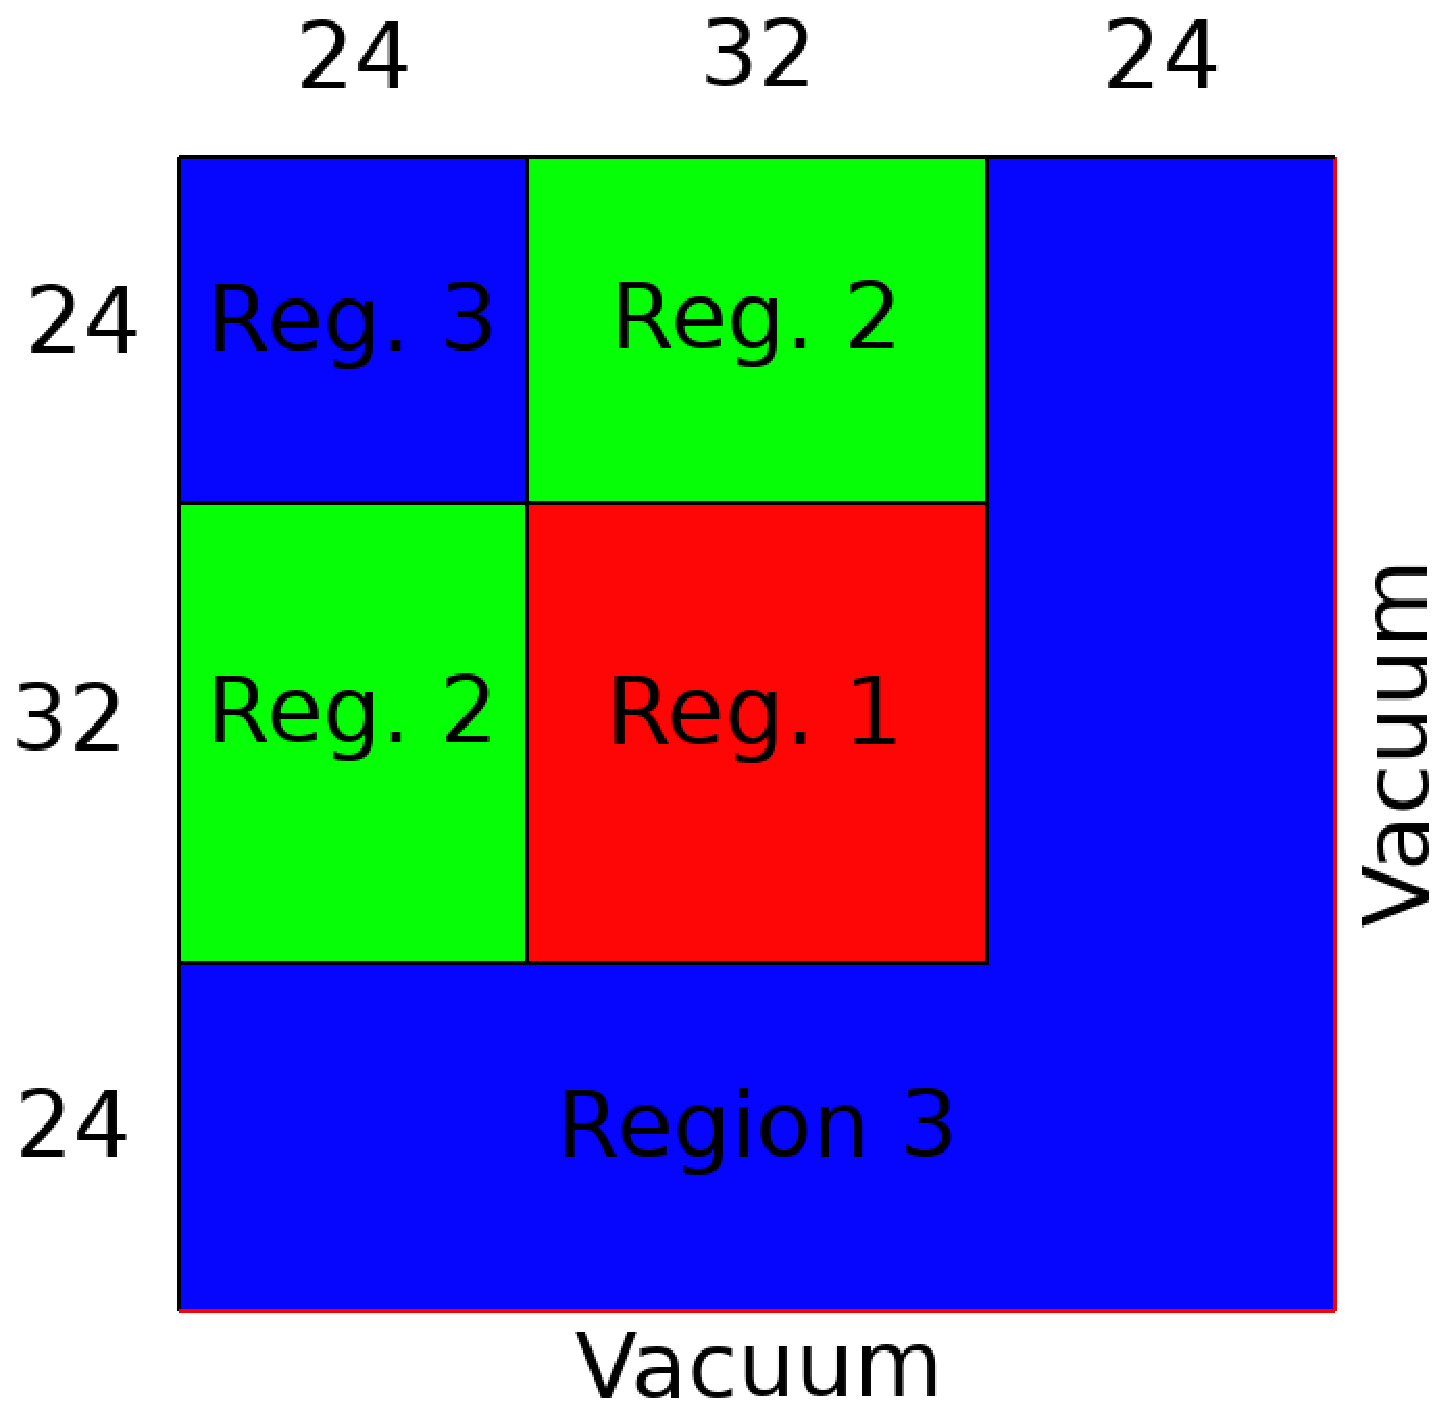
\includegraphics[width=0.4\linewidth]{twigl.eps}\\
	\caption{\label{image:canonsummary}Геометрическая модель 1/4 активной зоны теста TWIGL-2D.}
	\label{ris:twigl}
\end{center}
\end{figure}

Рассматривается двумерный транспортный тест \cite{hageman1969}. 
Моделируется 1/4 часть активной зоны реактора, размеры которой составляют 160x160 см.
На рисунке \ref{ris:twigl} показана геометрическая модель активной зоны, где цифрами показаны материалы различных сортов.
На внешней границе активной зоны реактора задается условие границы с вакуумом.  

Нейтронно-физические константы теста в общепринятых единицах представлены в таблице \ref{table:coeff}. 
Среднегрупповые скорости нейтронов в тесте одинаковы для всей среды и составляют $v_1 = 10^7$ см/с и $v_2 = 2 \cdot 10^5$ см/с. 
Спектр деления для мгновенных и запаздывающих нейтронов также одинаков для всей среды и равен $\chi_1 = 1$ и $\chi_2 = 0$.
В тесте представлена одна эффективная группа запаздывающих нейтронов. 
Эффективная доля запаздывающих нейтронов составляет $\beta = 0.0075$, а постоянная распада предшественников запаздывающих нейтронов $\lambda = 0.08$ с$^{-1}$. 

\begin{table}[ht]
\caption{\label{table:coeff}Диффузионные константы для теста TWIGL-2D.}
\label{t1}
\begin{center}
\begin{tabular}{rrrr}
\hline
Материал & 1 & 2 & 3\\
\hline 
$\Sigma_{t,1}$ 				& 0.2481 & 0.2481 & 0.2644 \\
$\Sigma_{t,2}$ 				& 0.9833 & 0.9833 & 0.7167 \\
$\Sigma_{a,1}$ 				& 0.01   & 0.01   & 0.008  \\
$\Sigma_{a,2}$ 				& 0.15   & 0.15   & 0.05   \\
$\Sigma_{s,1\rightarrow2}$ 	& 0.01   & 0.01   & 0.01   \\
$\Sigma_{s,1\rightarrow1}$ 	& 0.2281 & 0.2281 & 0.2464 \\
$\Sigma_{s,2\rightarrow2}$ 	& 0.8333 & 0.8333 & 0.6667 \\
$\nu_1\Sigma_{f,1}$ 		& 0.007  & 0.007  & 0.003  \\
$\nu_2\Sigma_{f,2}$ 		& 0.2    & 0.2    & 0.06   \\
\hline
\end{tabular}
\end{center}
\end{table}

Сценарий динамического процесса выглядит следующий образом:
\begin{itemize}\itemsep1pt \parskip0pt \parsep0pt
\item В начале решается $\lambda$-спектральная задача, решение которой принимается в качестве начального условия нестационарной задачи;
\item Расчет нестационарной задачи происходит в течении 0.5 секунд;
\item В каждый момент времени рассчитывается интегральная мощность
\begin{equation}\label{13}
P(t) = a\int_{\Omega}(\Sigma_{f,1} \phi_1 + \Sigma_{f,2} \phi_1) d\bm x,
\end{equation}
где $a$ --- нормировочный коэффициент, соответствующий заданному значению интегральной мощности.
\end{itemize}

Все возмущения происходят в зоне 1 посредством изменения теплового сечения деления $\Sigma_{a2}$.
В задаче представлены три сценария развития переходного процесса:
\begin{itemize}\itemsep1pt \parskip0pt \parsep0pt
\item Скачкообразное возмущение TWIGL-S: инициируется уменьшением $\Sigma_{a2}$ на $0.0035$ см$^{-1}$ в нулевой момент времени;
\item Линейное возмущение TWIGL-R: $\Sigma_{a2}$ линейно уменьшается на $0.0035$ см$^{-1}$ с момента времени $0$ секунд до $0.2$ секунд;
\item Комбинированное возмущение TWIGL-C происходит следующим образом:
$\Sigma_{a2}$ линейно уменьшается на $0.0035$ см$^{-1}$ в течении $0.2$ секунд; в момент времени $0.2$ секунд происходит скачкообразное увеличение на $0.00525$ см$^{-1}$; линейно увеличивается на $0.00175$ см$^{-1}$  с момента времени $0.2$ секунд до $0.4$ секунд;  скачкообразное уменьшение на $0.0035$ см$^{-1}$ в момент времени $0.4$ секунд.
\end{itemize}
 
В комбинированном случае представлены другие параметры для запаздывающих нейтронов: $v_1 = 10^7$ см/с и $v_2 = 10^5$ см/с; эффективная доля запаздывающих нейтронов составляет $\beta = 0.0064$;  постоянная распада предшественников запаздывающих нейтронов $\lambda = 0.08$ с$^{-1}$. 

\subparagraph{Решение $\lambda$-спектральной задачи}
В качестве эталонного решения для $\lambda$-спектральной задачи выступает результат полученный методом Монте-Карло по коду DeCART равный $0.91605$ (\cite{joo2004}).
Полученные результаты расчета $\lambda$-спектральной задачи для теста TWIGL-2D приведены в таблице \ref{table:t2-lamda}.
В таблице приняты следующие обозначения: 
$k_{dif}$ --- эффективный коэффициент размножения по диффузионной модели; 
$k_{sp_3}$ --- эффективный коэффициент размножения по транспортной SP$_3$ модели;
$\Delta$ --- абсолютное отклонение от эталонного решения в pcm ($10^{-5}$).

\begin{table}[h]
\caption{Результаты расчета $\lambda$-спектральной задачи.}
\label{table:t2-lamda}
\begin{center}
\begin{tabular}{r r r r r r}
\hline
$n$ & $p$ & $k_{dif}$ & $\Delta_{dif}$ & $k_{sp_3}$ & $\Delta_{sp3}$\\
\hline
	& 1	& 0.91552 & -53& 0.91614 & 9 \\
2	& 2	& 0.91552 & -53& 0.91619 &14 \\
	& 3	& 0.91542 & -63& 0.91609 & 4 \\ 
\hline
	& 1	& 0.91549 & -56& 0.91615 & 10\\
8& 2	& 0.91542 & -63& 0.91610 & 5 \\
	& 3	& 0.91541 & -64& 0.91608 & 3 \\ 
\hline
	& 1	& 0.91543 & -62& 0.91610 & 5 \\
32& 2	& 0.91541 & -64& 0.91608 & 3 \\
	& 3	& 0.91541 & -64& 0.91607 & 2 \\
\hline
ref.&   & 0.91605 & -- & 0.91605 & --\\
\hline
\end{tabular}
\end{center}
\end{table}

Представленные данные демонстрируют сходимость приближенно вычисляемых собственных значений при сгущении вычислительной сетки $n$ и при увеличении степени полиномов конечных элементов $p$.
На рисунке \ref{ris:int_pwr} показаны расчеты нормированных мощностей (\ref{13}) по нодам 8х8 см на мелкой сетке $n=32$ и $p=3$, где жирным выделено эталонное решение полученное по коду DeCART.
Как и ожидалось, точность результатов полученных транспортным SP$_3$ методом, выше по сравнению с диффузионным расчетом.

\begin{figure}[ht]
\begin{center}
	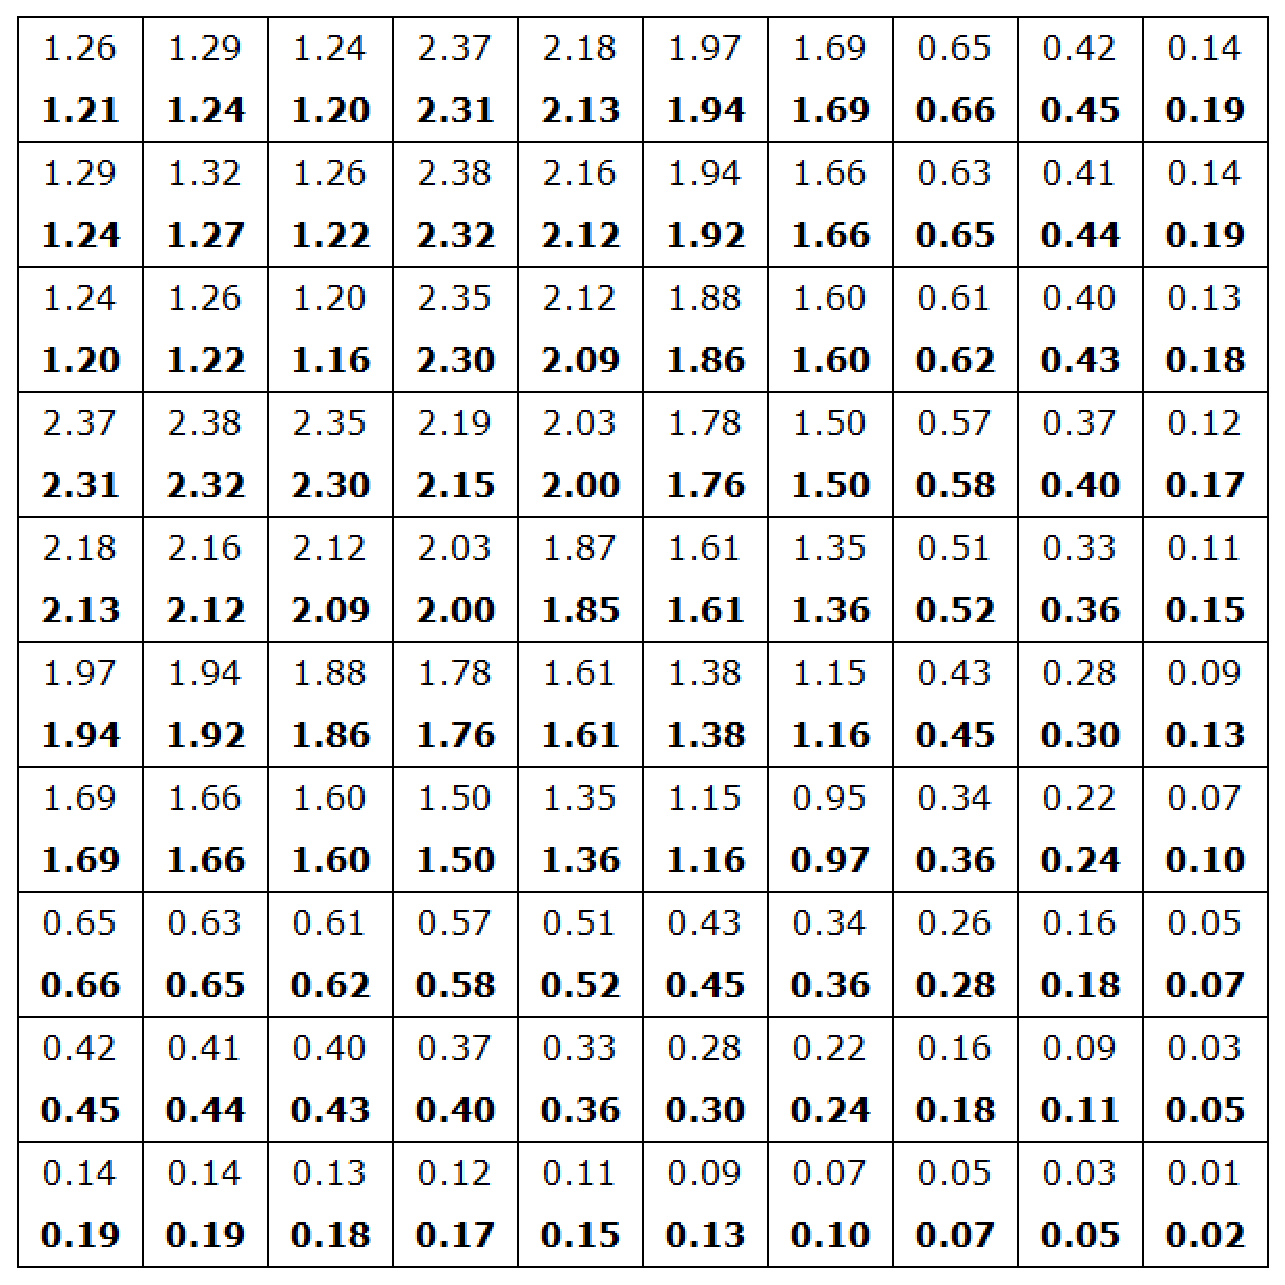
\includegraphics[width=0.4\linewidth]{dif_pwr.eps} \hspace{20pt}
	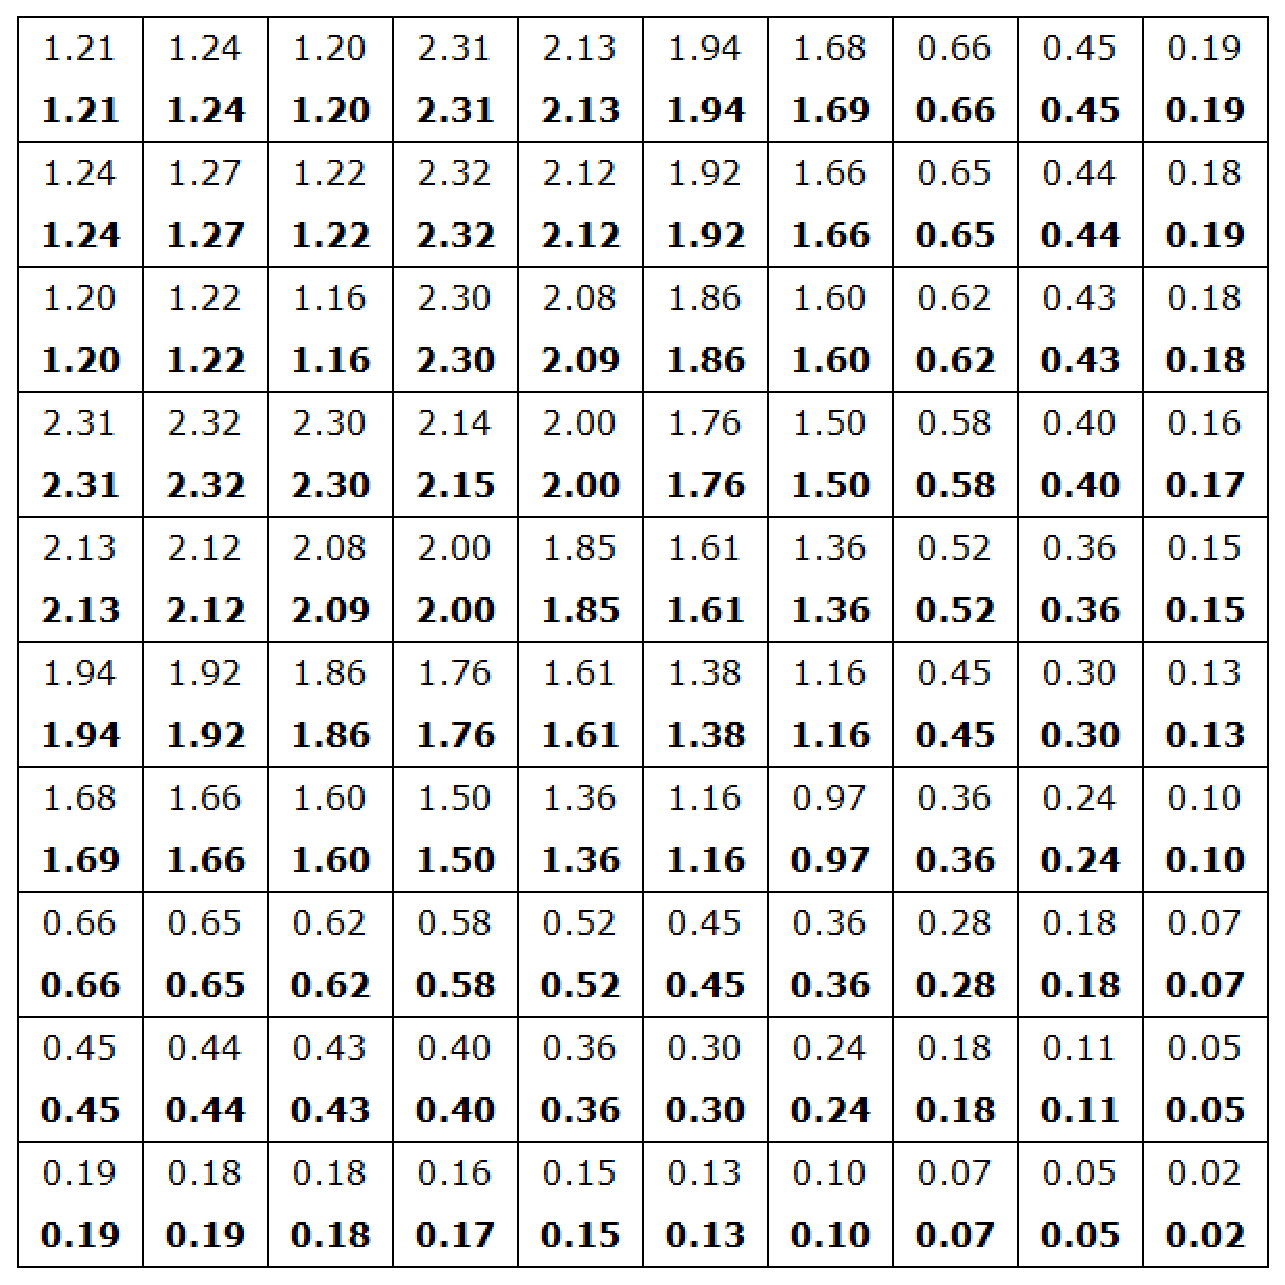
\includegraphics[width=0.4\linewidth]{sp3_pwr.eps}\\
	\caption{\label{image:canonsummary} Нормированная мощность диффузионного расчета (слева) и транспортного SP$_3$ расчета (справа) на мелкой сетке, жирным --- эталонное решение.}
	\label{ris:int_pwr}
\end{center}
\end{figure}

\subparagraph{Решение нестационарной задачи}
Здесь показаны результаты решений нестационарной задачи для всех трех сценариев.
Шаг по времени $\tau=1$ мс.
Проводится сравнение результатов диффузионного и транспортного расчетов.
Эталонными решениями выступают результаты полученные транспортными кодами DORT-TD, MGSNM (метод дискретных ординат) и транспортными кодами DeCART, MPACT (метод характеристик) \cite{kondrushin2014}.

Представлены исследования различных шагов по времени для всех трех сценариев.  
Для исследования сходимости численного решения, в качестве тестовой сетки  по пространству выбран средний вариант вычислительной сетки при $n=8,\ p=2$.
Погрешность оценивается как $\varepsilon_P(t) = | P_{ref} - P |$, где $P_{ref}$ --- эталонное решение.

\subparagraph{Сценарий №1: скачкообразное возмущение}
В таблице \ref{table:twigl-s} представлены результаты диффузионного и транспортного расчетов TWIGL-S в различные моменты времени на мелкой сетке.
На рисунке \ref{ris:sp3_ref_s} показаны транспортное SP$_3$ решение и погрешность $\varepsilon_P$ диффузионного решения относительно транспортного решения на мелкой сетке. 

\begin{table}[ht]
\caption{Результаты расчетов TWIGL-S на мелкой сетке в различные моменты времени.}
\label{table:twigl-s}
\begin{center}
\begin{tabular}{c c c c c}
\hline
$t$ & dif & SP$_3$ & DORT-TD & MGSNM \\
\hline
0.0 & 1.000 & 1.000 & 1.000 & 1.000 \\
0.1 & 2.078 & 2.090 & 2.091 & 2.093 \\
0.2 & 2.096 & 2.108 & 2.109 & 2.110 \\
0.3 & 2.114 & 2.126 & 2.127 & 2.128 \\
0.4 & 2.132 & 2.144 & 2.144 & 2.145 \\
0.5 & 2.150 & 2.163 & 2.163 & 2.163 \\
\hline
время счета & 2000 & 6500  \\
\end{tabular}
\end{center}
\end{table}

На рисунке \ref{ris:tau_s} представлена погрешность $\varepsilon_P$ диффузионных/транспортных расчетов на тестовой сетке при различных шагах по времени. 
Полученные результаты демонстрируют сходимость решения при уменьшении шага по времени.

\begin{figure}[ht]
\begin{center}
	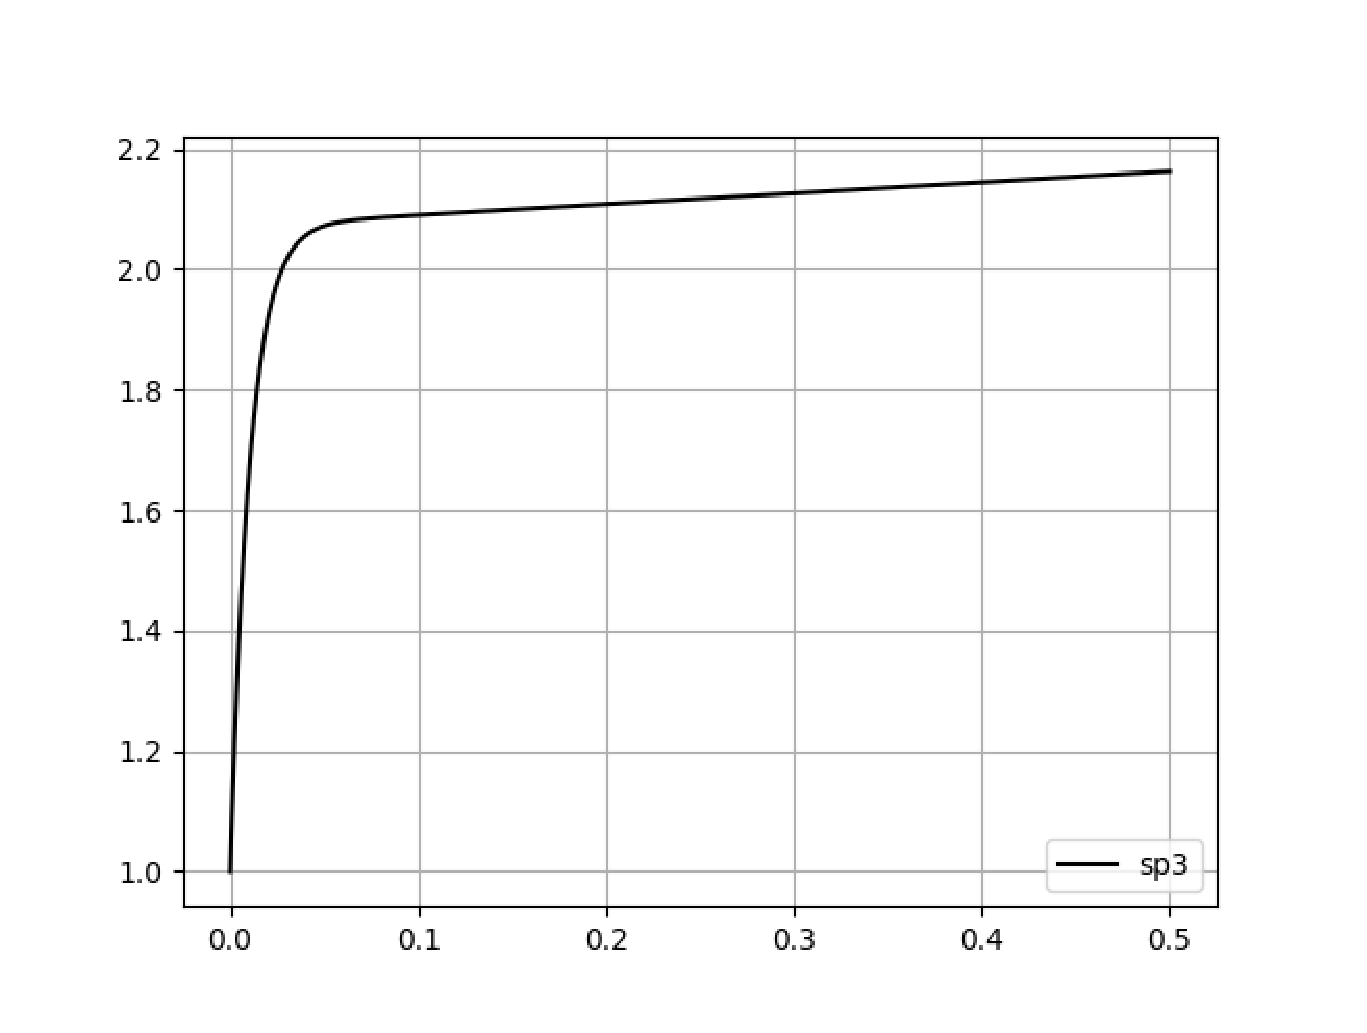
\includegraphics[width=0.4\linewidth]{sp3_ref_s.eps}\hspace{20pt}
	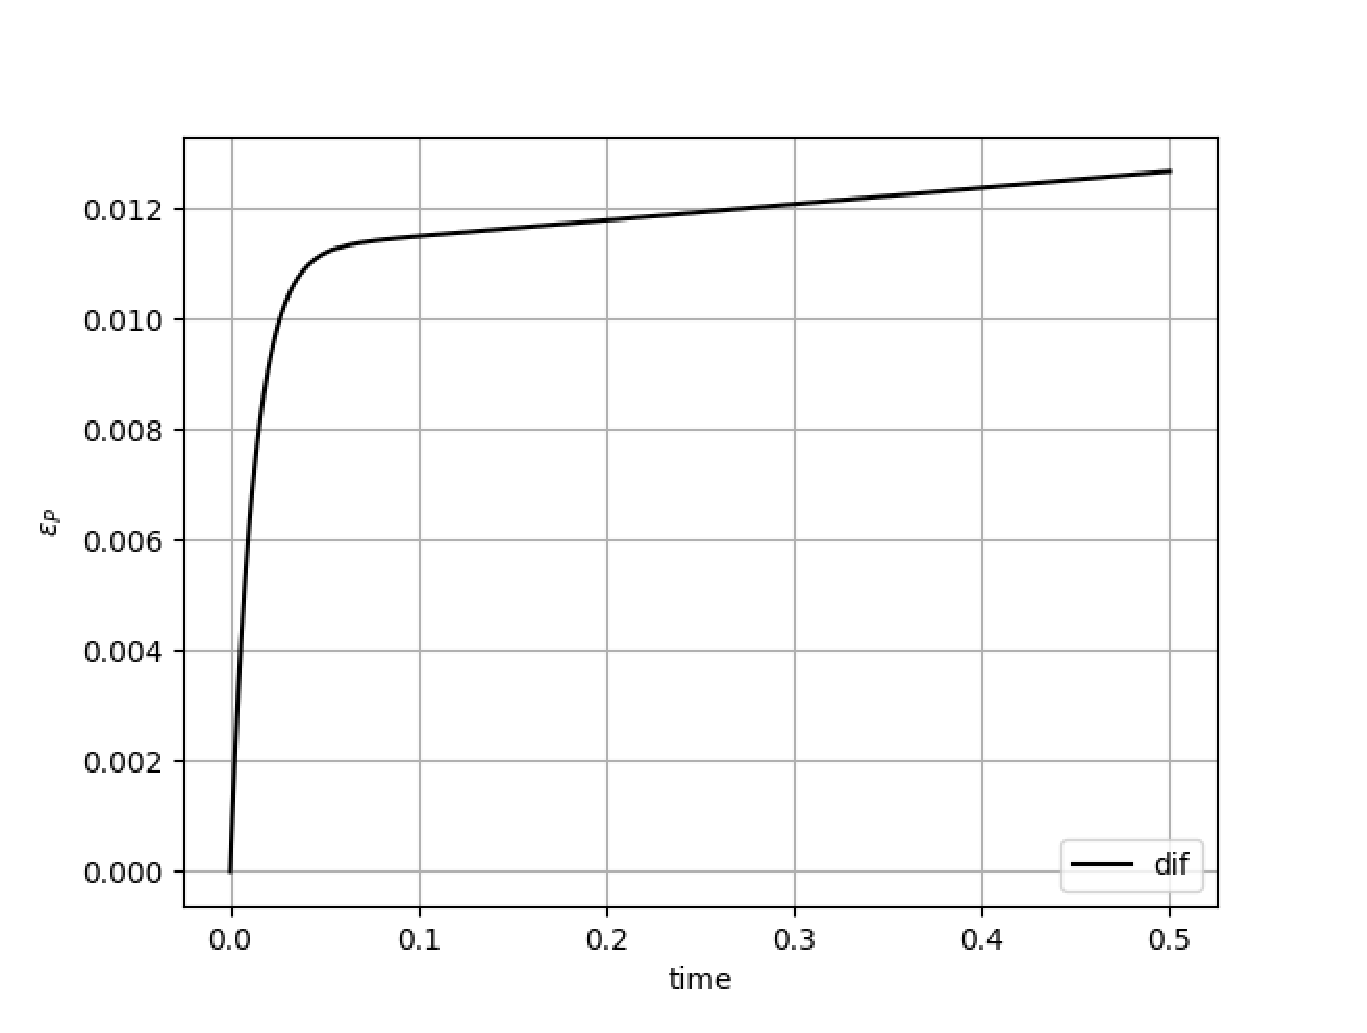
\includegraphics[width=0.4\linewidth]{odds_s.eps}\\
	\caption{\label{image:canonsummary} Транспортное SP$_3$ решение TWIGL-S (слева) и погрешность $\varepsilon_P$ диффузионного расчета (справа) на мелкой сетке.}
	\label{ris:sp3_ref_s}
\end{center}
\end{figure}

\begin{figure}[ht]
\begin{center}
	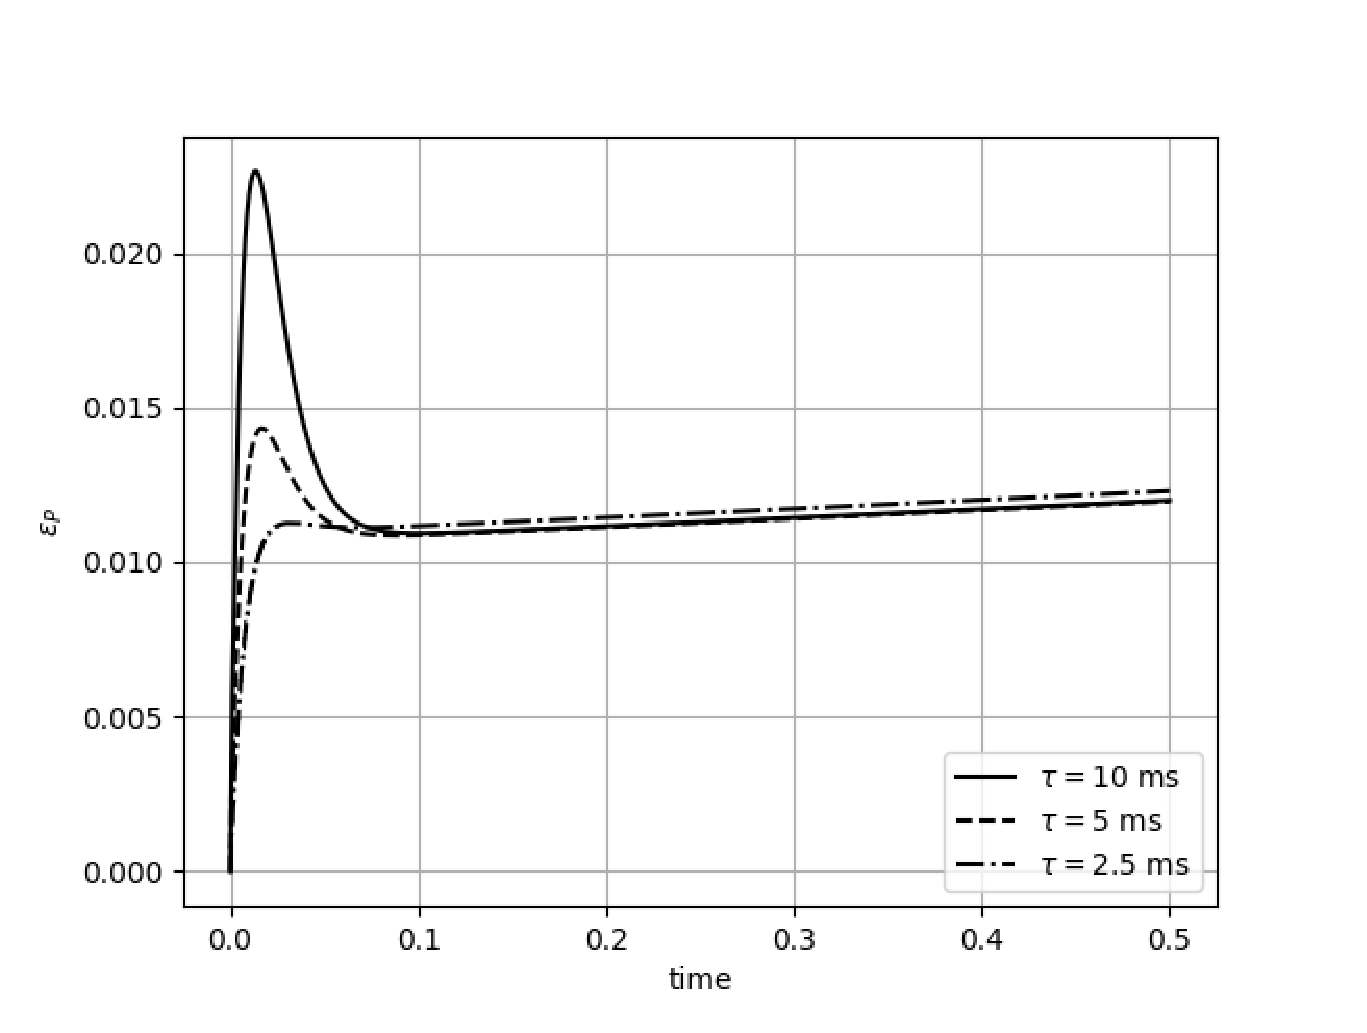
\includegraphics[width=0.4\linewidth]{dif_tau_s.eps}\hspace{20pt}
	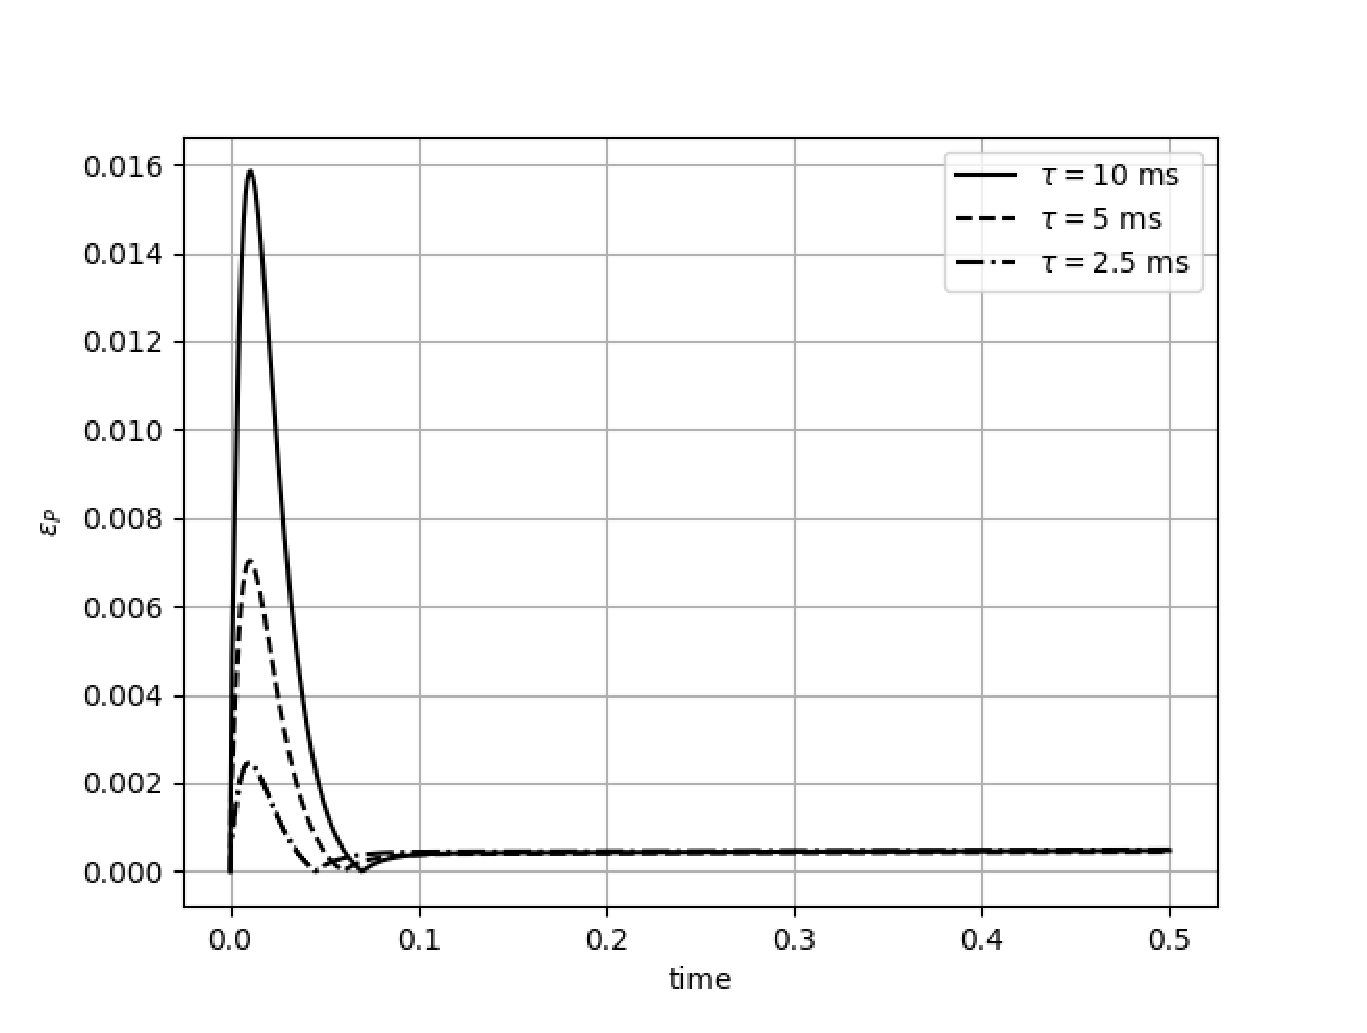
\includegraphics[width=0.4\linewidth]{sp3_tau_s.eps}\\
	\caption{\label{image:canonsummary} Погрешность $\varepsilon_P$ диффузионного расчета (слева) и транспортного SP$_3$ расчета (справа) для тестовой сетки TWIGL-S при различных шагах по времени.}
	\label{ris:tau_s}
\end{center}
\end{figure}

\subparagraph{Cценарий №2: линейное возмущение}
В таблице \ref{table:twigl-r} представлены результаты диффузионного и транспортного расчетов TWIGL-S в различные моменты времени на мелкой сетке.
На рисунке \ref{ris:sp3_ref_r} показаны транспортное SP$_3$ решение и погрешность $\varepsilon_P$ диффузионного решения относительно транспортного решения на мелкой сетке. 

\begin{table}[ht]
\caption{Результаты расчетов TWIGL-R на мелкой сетке в различные моменты времени.}
\label{table:twigl-r}
\begin{center}
\begin{tabular}{c c c c c}
\hline
$t$ & Dif & SP$_3$ & DORT-TD & MGSNM \\
\hline
0.0 & 1.000 & 1.000 & 1.000 & 1.000\\
0.1 & 1.311 & 1.313 & 1.314 & 1.315\\
0.2 & 1.973 & 1.983 & 1.984 & 1.984\\
0.3 & 2.092 & 2.104 & 2.102 & 2.102\\
0.4 & 2.110 & 2.122 & 2.123 & 2.124\\
0.5 & 2.128 & 2.140 & 2.140 & 2.141\\
\hline
время счета & 2000 & 6500 \\
\end{tabular}
\end{center}
\end{table}

\begin{figure}[ht]
\begin{center}
	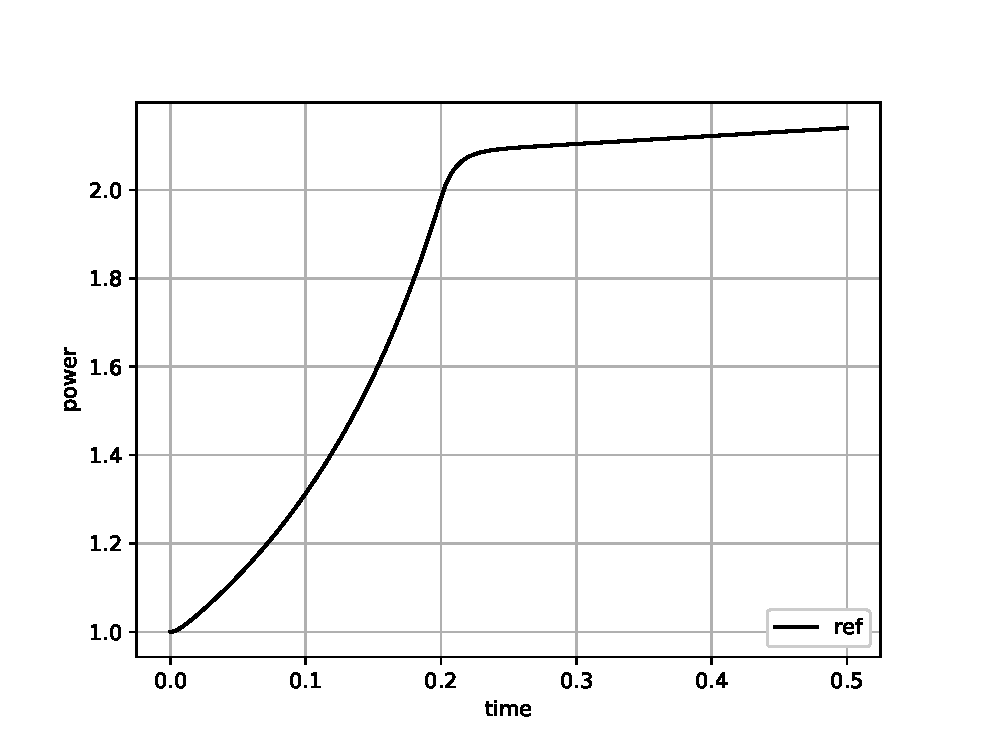
\includegraphics[width=0.4\linewidth]{sp3_ref_r.eps}\hspace{20pt}
	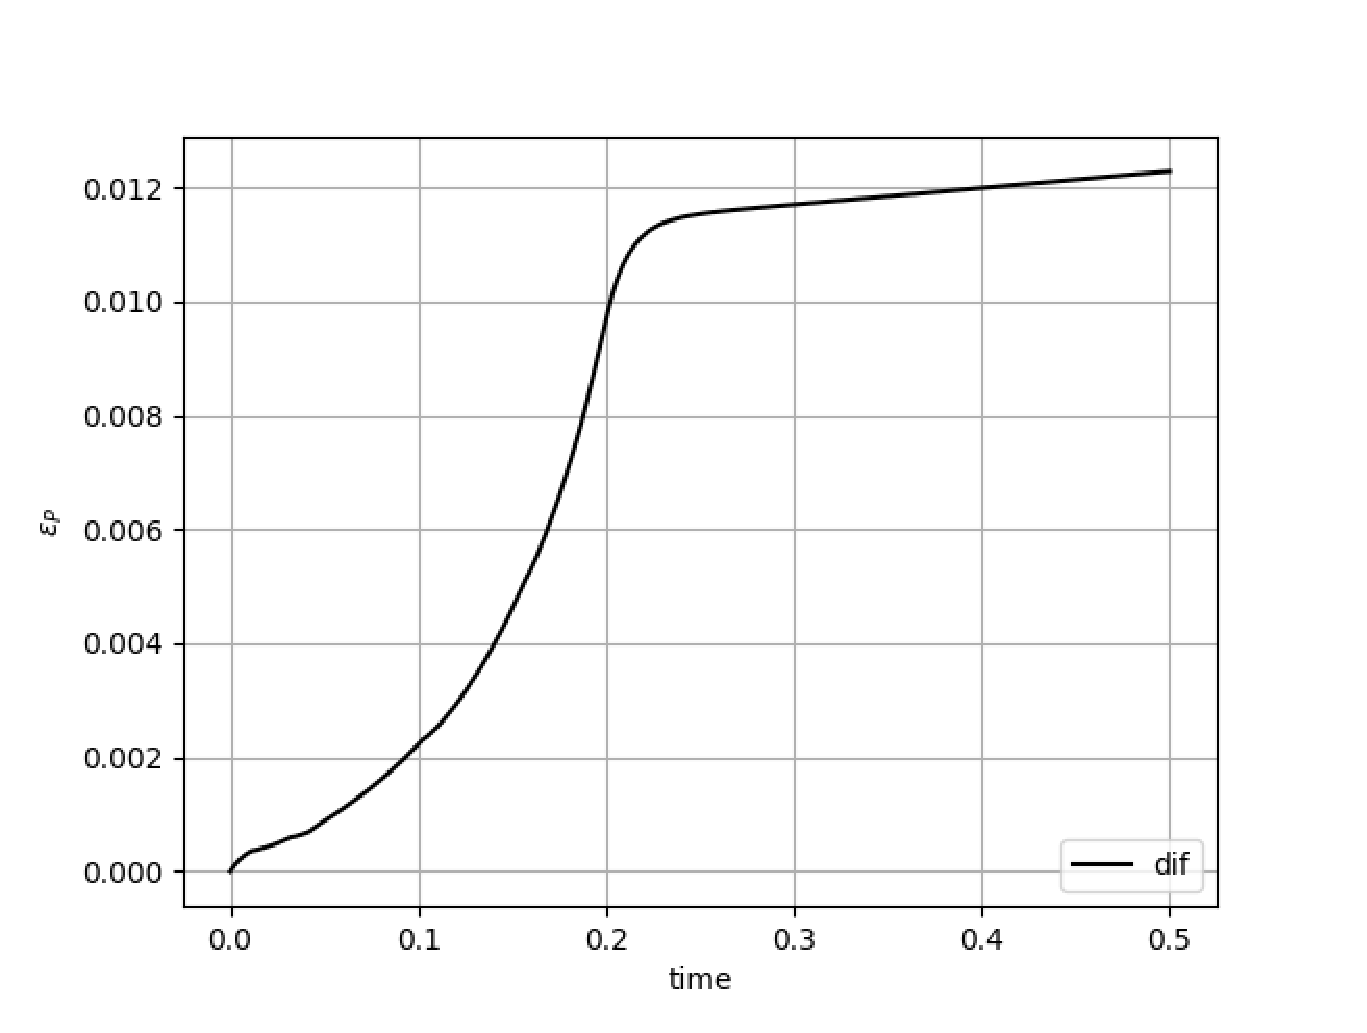
\includegraphics[width=0.4\linewidth]{odds_r.eps}\\
	\caption{\label{image:canonsummary} Транспортное SP$_3$ решение TWIGL-R (слева) и погрешность $\varepsilon_P$ диффузионного расчета (справа) на мелкой сетке. }
	\label{ris:sp3_ref_r}
\end{center}
\end{figure}

На рисунке \ref{ris:tau_r} представлена погрешность $\varepsilon_P$ диффузионных/транспортных расчетов на тестовой сетке при различных шагах по времени. 
Полученные результаты демонстрируют сходимость решения при уменьшении шага по времени.

\begin{figure}[ht]
\begin{center}
	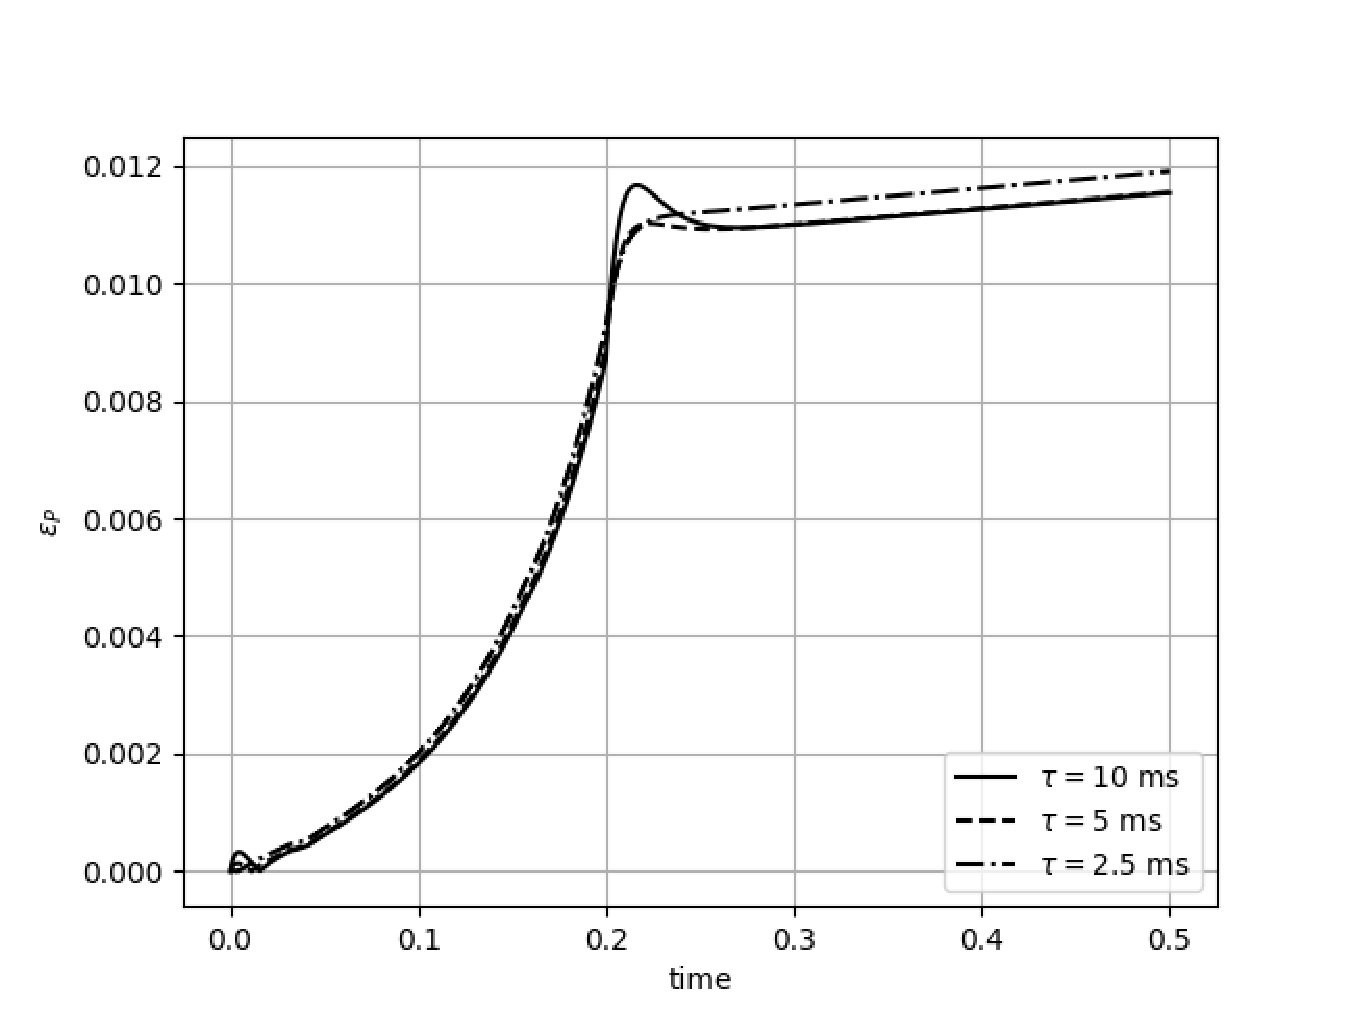
\includegraphics[width=0.4\linewidth]{dif_tau_r.eps}\hspace{20pt}
	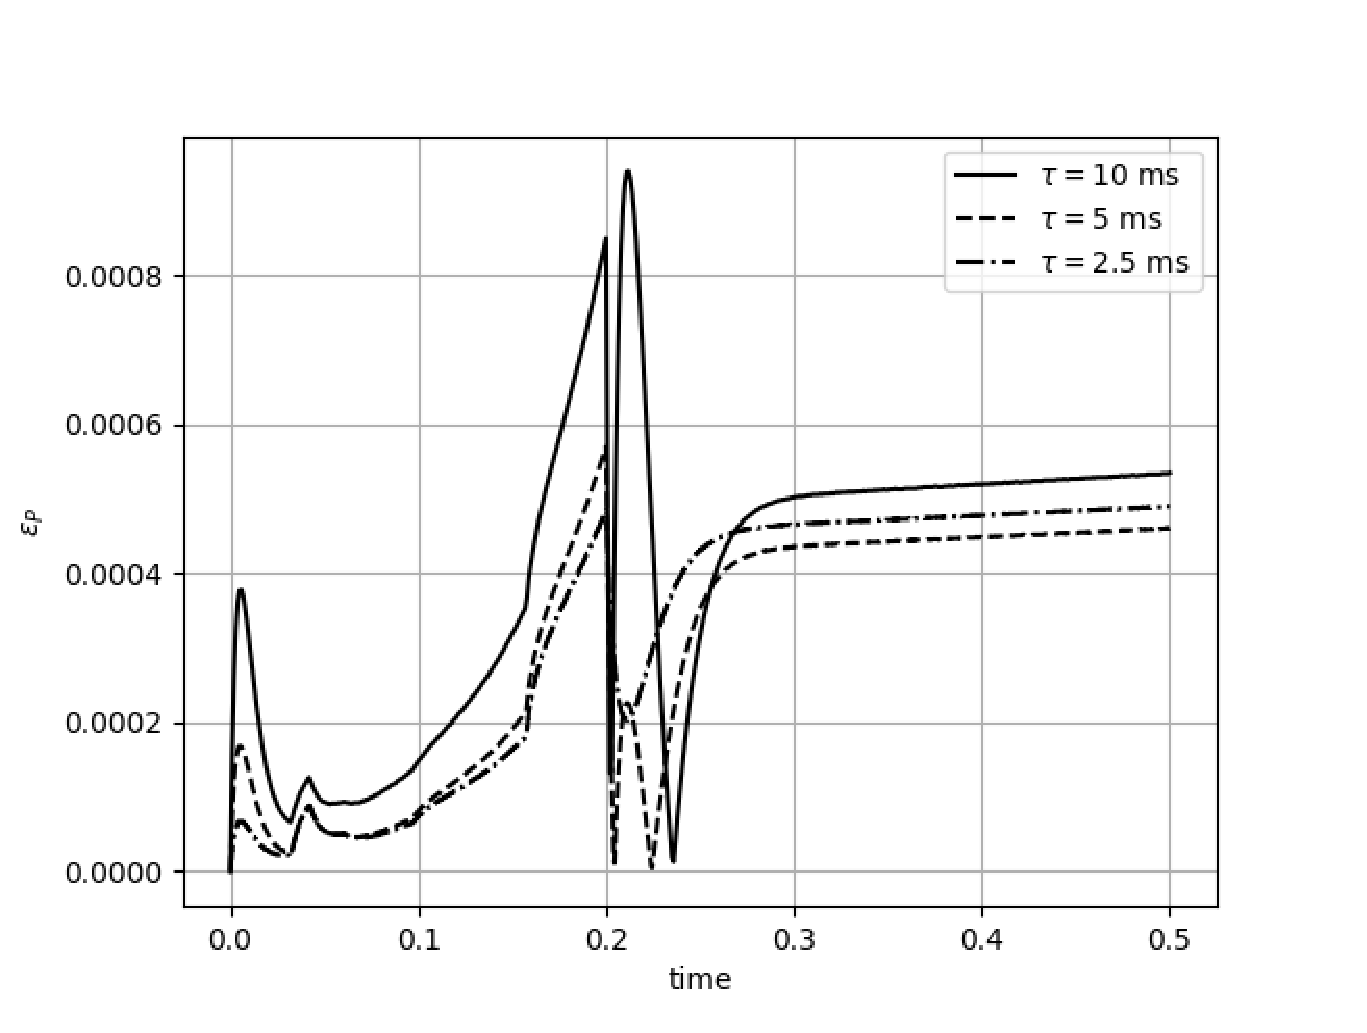
\includegraphics[width=0.4\linewidth]{sp3_tau_r.eps}\\
	\caption{\label{image:canonsummary} Погрешность $\varepsilon_P$ диффузионного расчета (слева) и транспортного SP$_3$ расчета (справа) для тестовой сетки TWIGL-R при различных шагах по времени.}
	\label{ris:tau_r}
\end{center}
\end{figure}

\subparagraph{Cценарий №3: комбинированное возмущение}
\begin{table}[htp]
\caption{Результаты расчетов TWIGL-C на мелкой сетке в различные моменты времени.}
\label{table:twigl-c}
\begin{center}
\begin{tabular}{c c c c c}
\hline
$t$ & Dif & SP$_3$ & DeCART & MPACT\\
\hline
0.0 & 1.000 & 1.000 & 1.000 & 1.000 \\
0.1 & 1.342 & 1.340 & 1.341 & 1.342 \\
0.2 & 2.167 & 2.176 & 2.183 & 2.189 \\
0.3 & 0.710 & 0.711 & 0.715 & 0.716 \\
0.4 & 0.645 & 0.645 & 0.640 & 0.638 \\
0.5 & 1.002 & 1.005 & 1.002 & 1.003 \\
\hline
время счета & 2000 & 6500 \\
\end{tabular}
\end{center}
\end{table}
\begin{figure}[ht]
\begin{center}
	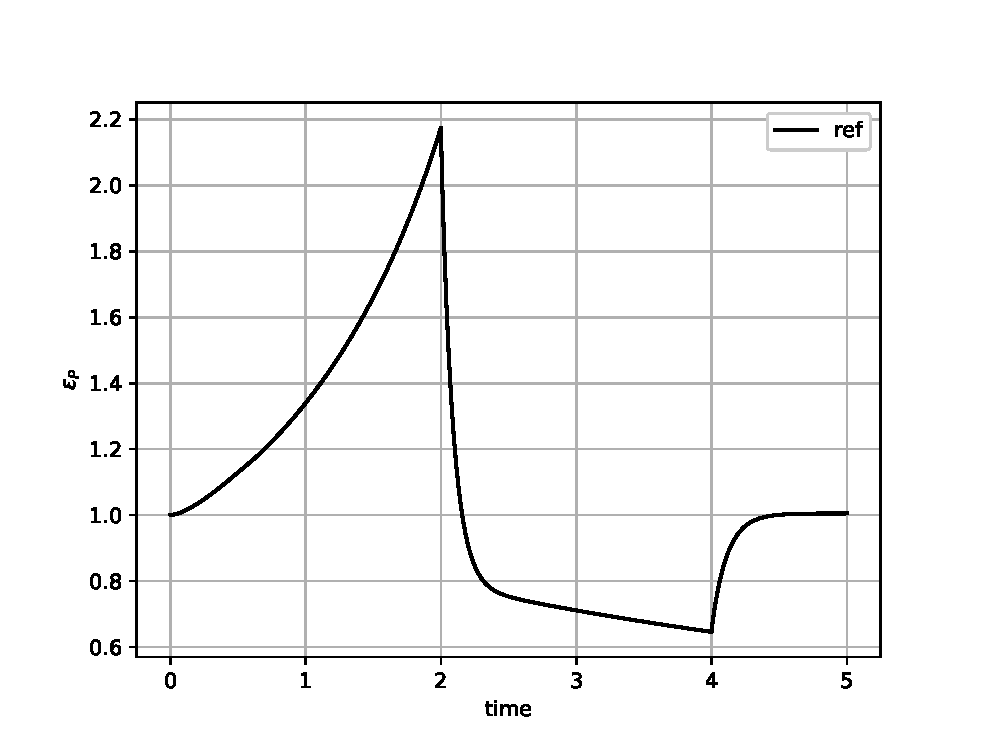
\includegraphics[width=0.4\linewidth]{sp3_ref_c.eps}\hspace{20pt}
	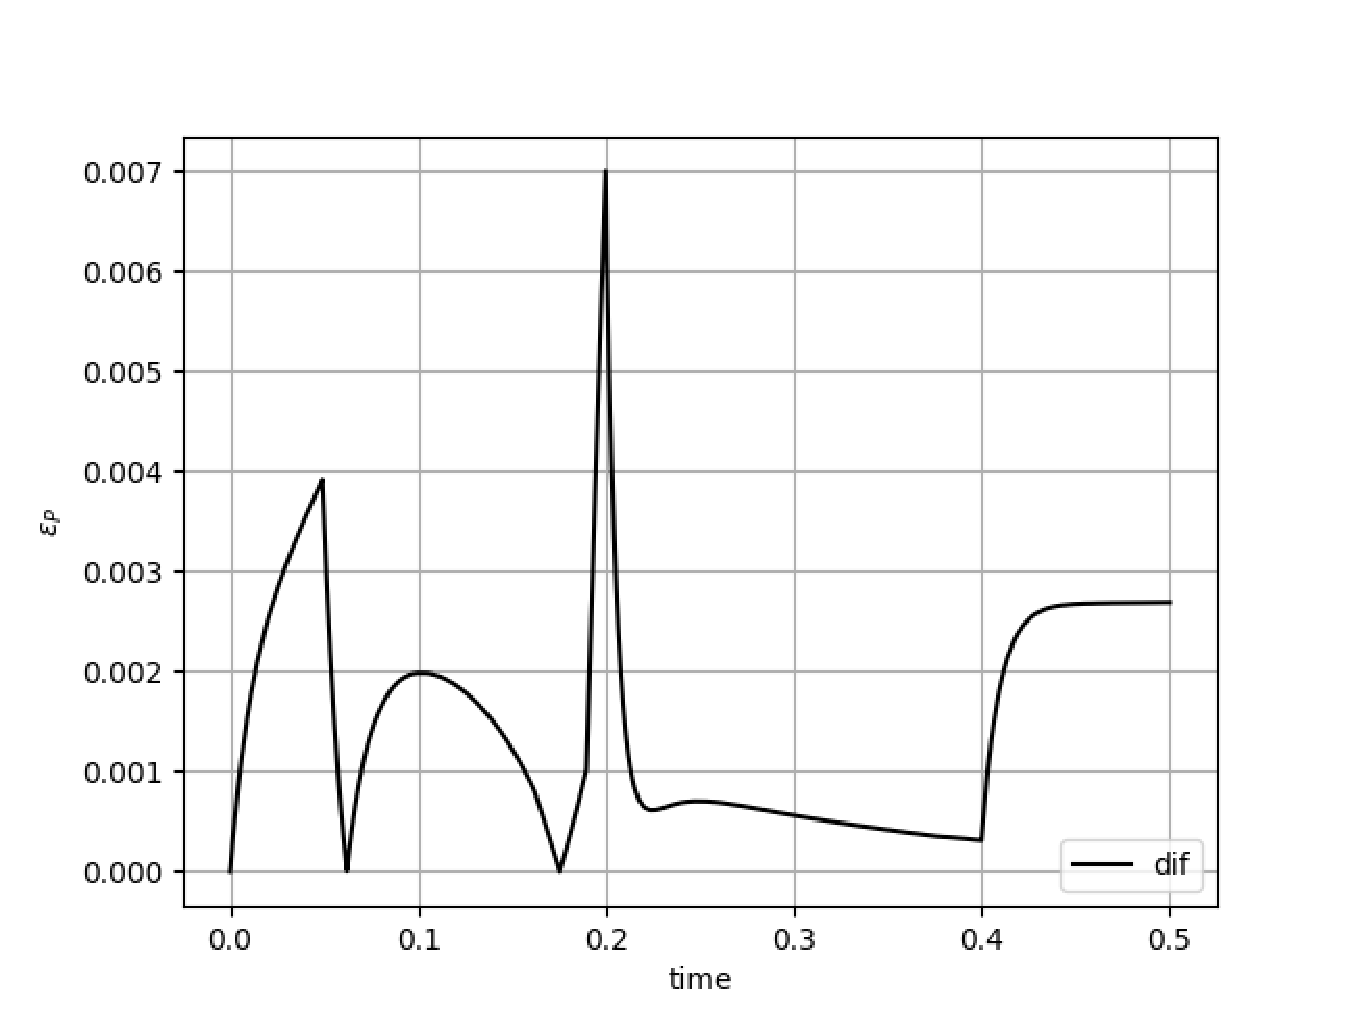
\includegraphics[width=0.4\linewidth]{odds_c.eps}\\
	\caption{\label{image:canonsummary} Транспортное SP$_3$ решение TWIGL-C (слева) и погрешность $\varepsilon_P$ диффузионногог расчета (справа) на мелкой сетке. }
	\label{ris:sp3_ref_c}
\end{center}
\end{figure}

В таблице \ref{table:twigl-c} представлены результаты диффузионного и транспортного расчетов TWIGL-S в различные моменты времени на мелкой сетке.
На рисунке \ref{ris:sp3_ref_c} показаны транспортное SP$_3$ решение и погрешность $\varepsilon_P$ диффузионного решения относительно транспортного решения на мелкой сетке. 

\begin{figure}[ht]
\begin{center}
	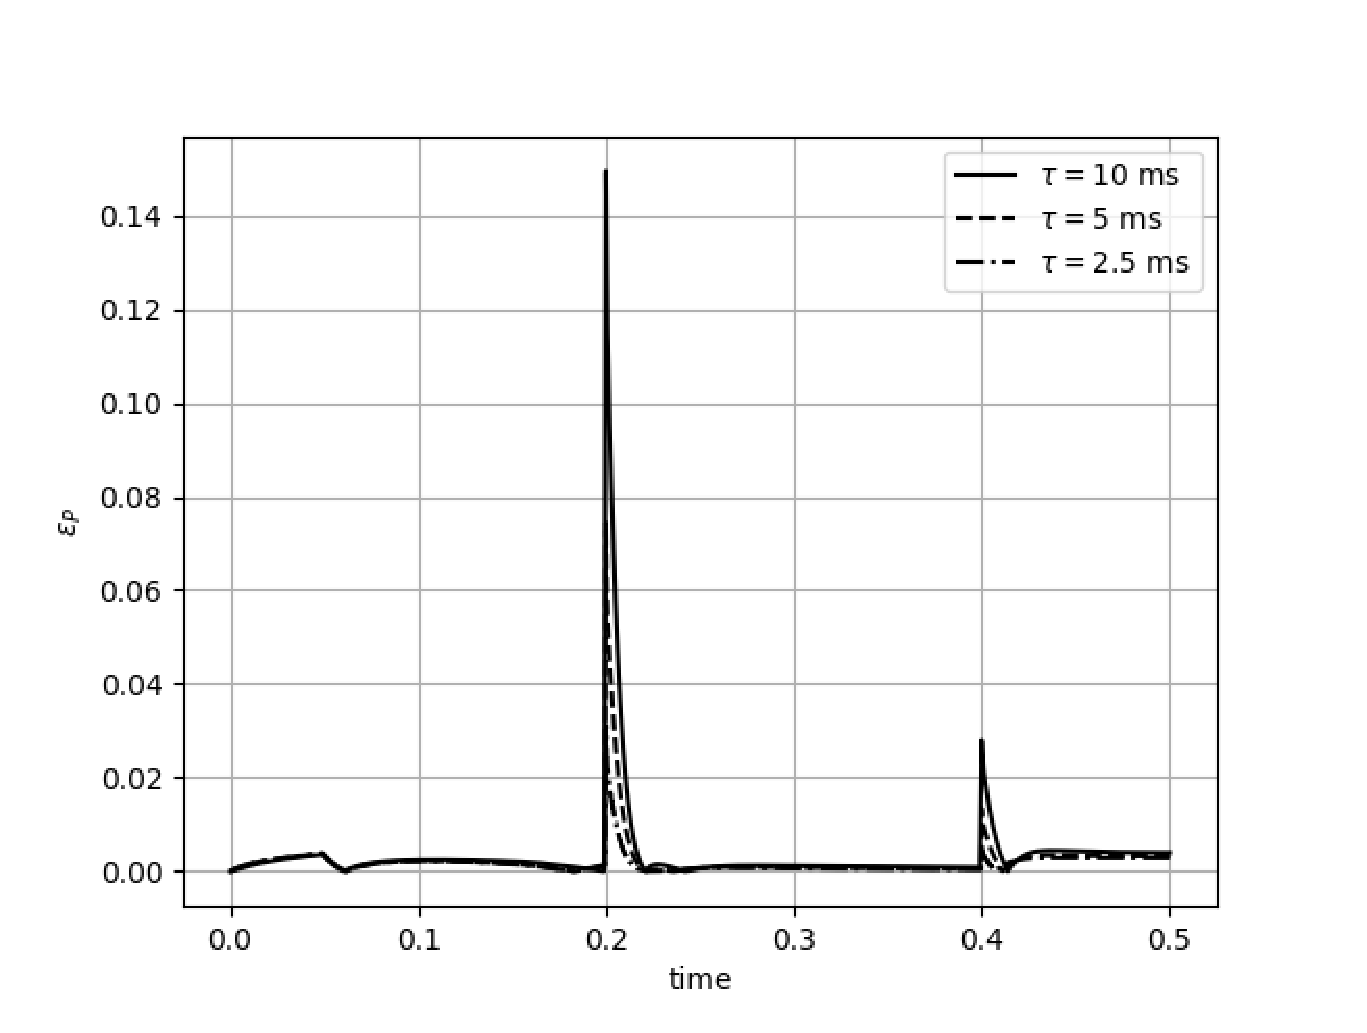
\includegraphics[width=0.4\linewidth]{dif_tau_c.eps}\hspace{20pt}
	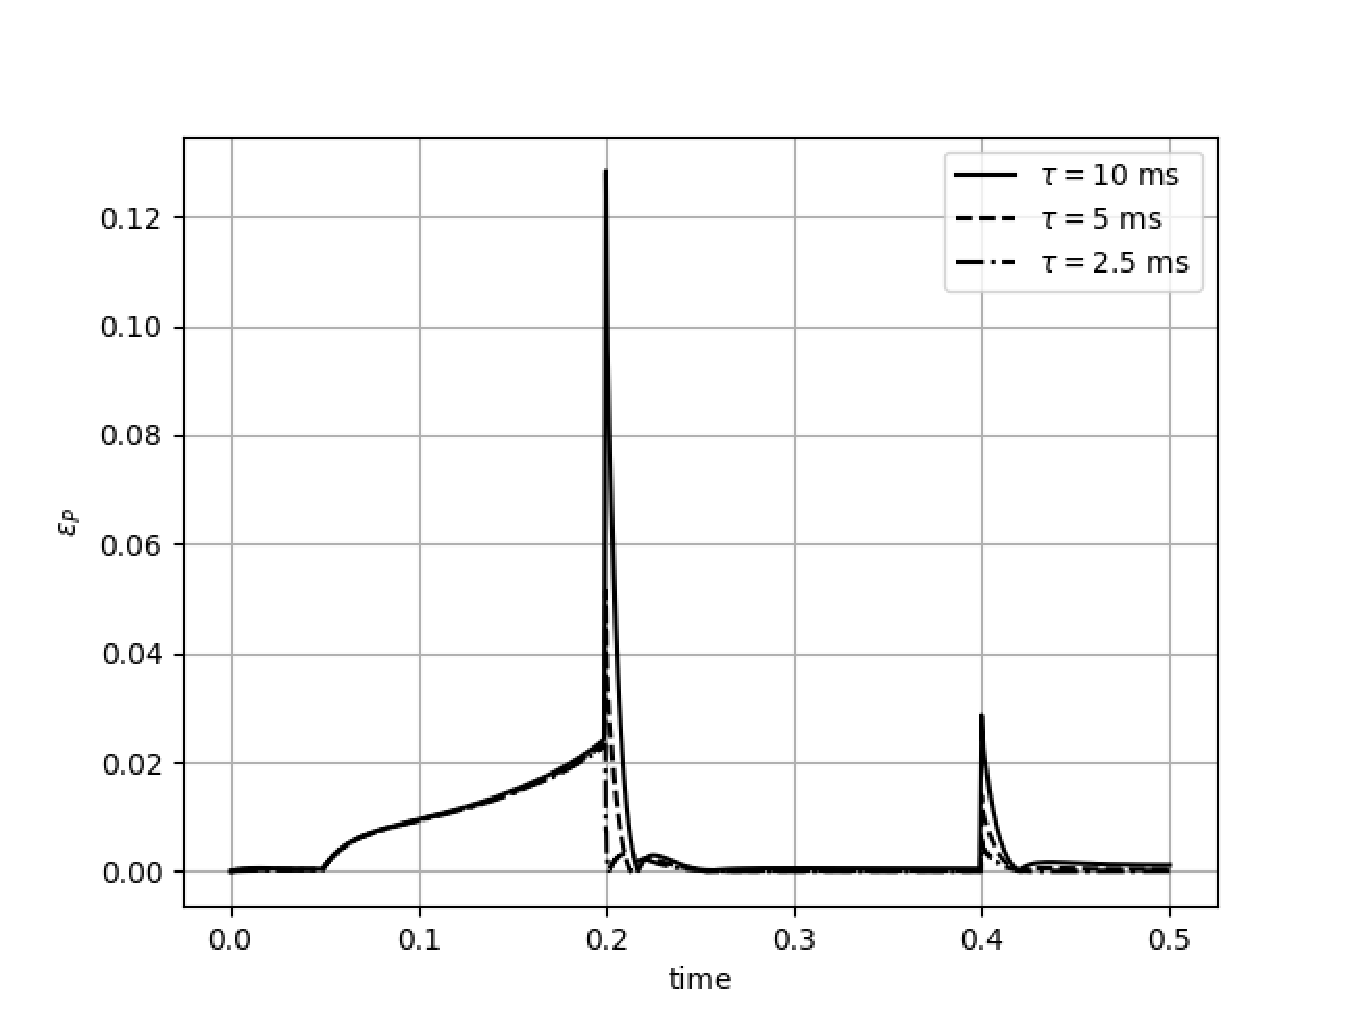
\includegraphics[width=0.4\linewidth]{sp3_tau_c.eps}\\
	\caption{\label{image:canonsummary} Погрешность $\varepsilon_P$ диффузионного расчета (слева) и  транспортного SP$_3$ расчета (справа) для тестовой сетки TWIGL-C при различных шагах по времени.}
	\label{ris:tau_c}
\end{center}
\end{figure}

На рисунке \ref{ris:tau_c} представлена погрешность $\varepsilon_P$ диффузионных/транспортных расчетов на тестовой сетке при различных шагах по времени. 
Полученные результаты демонстрируют сходимость решения при уменьшении шага по времени. 

\begin{figure}[h]
\begin{center}
	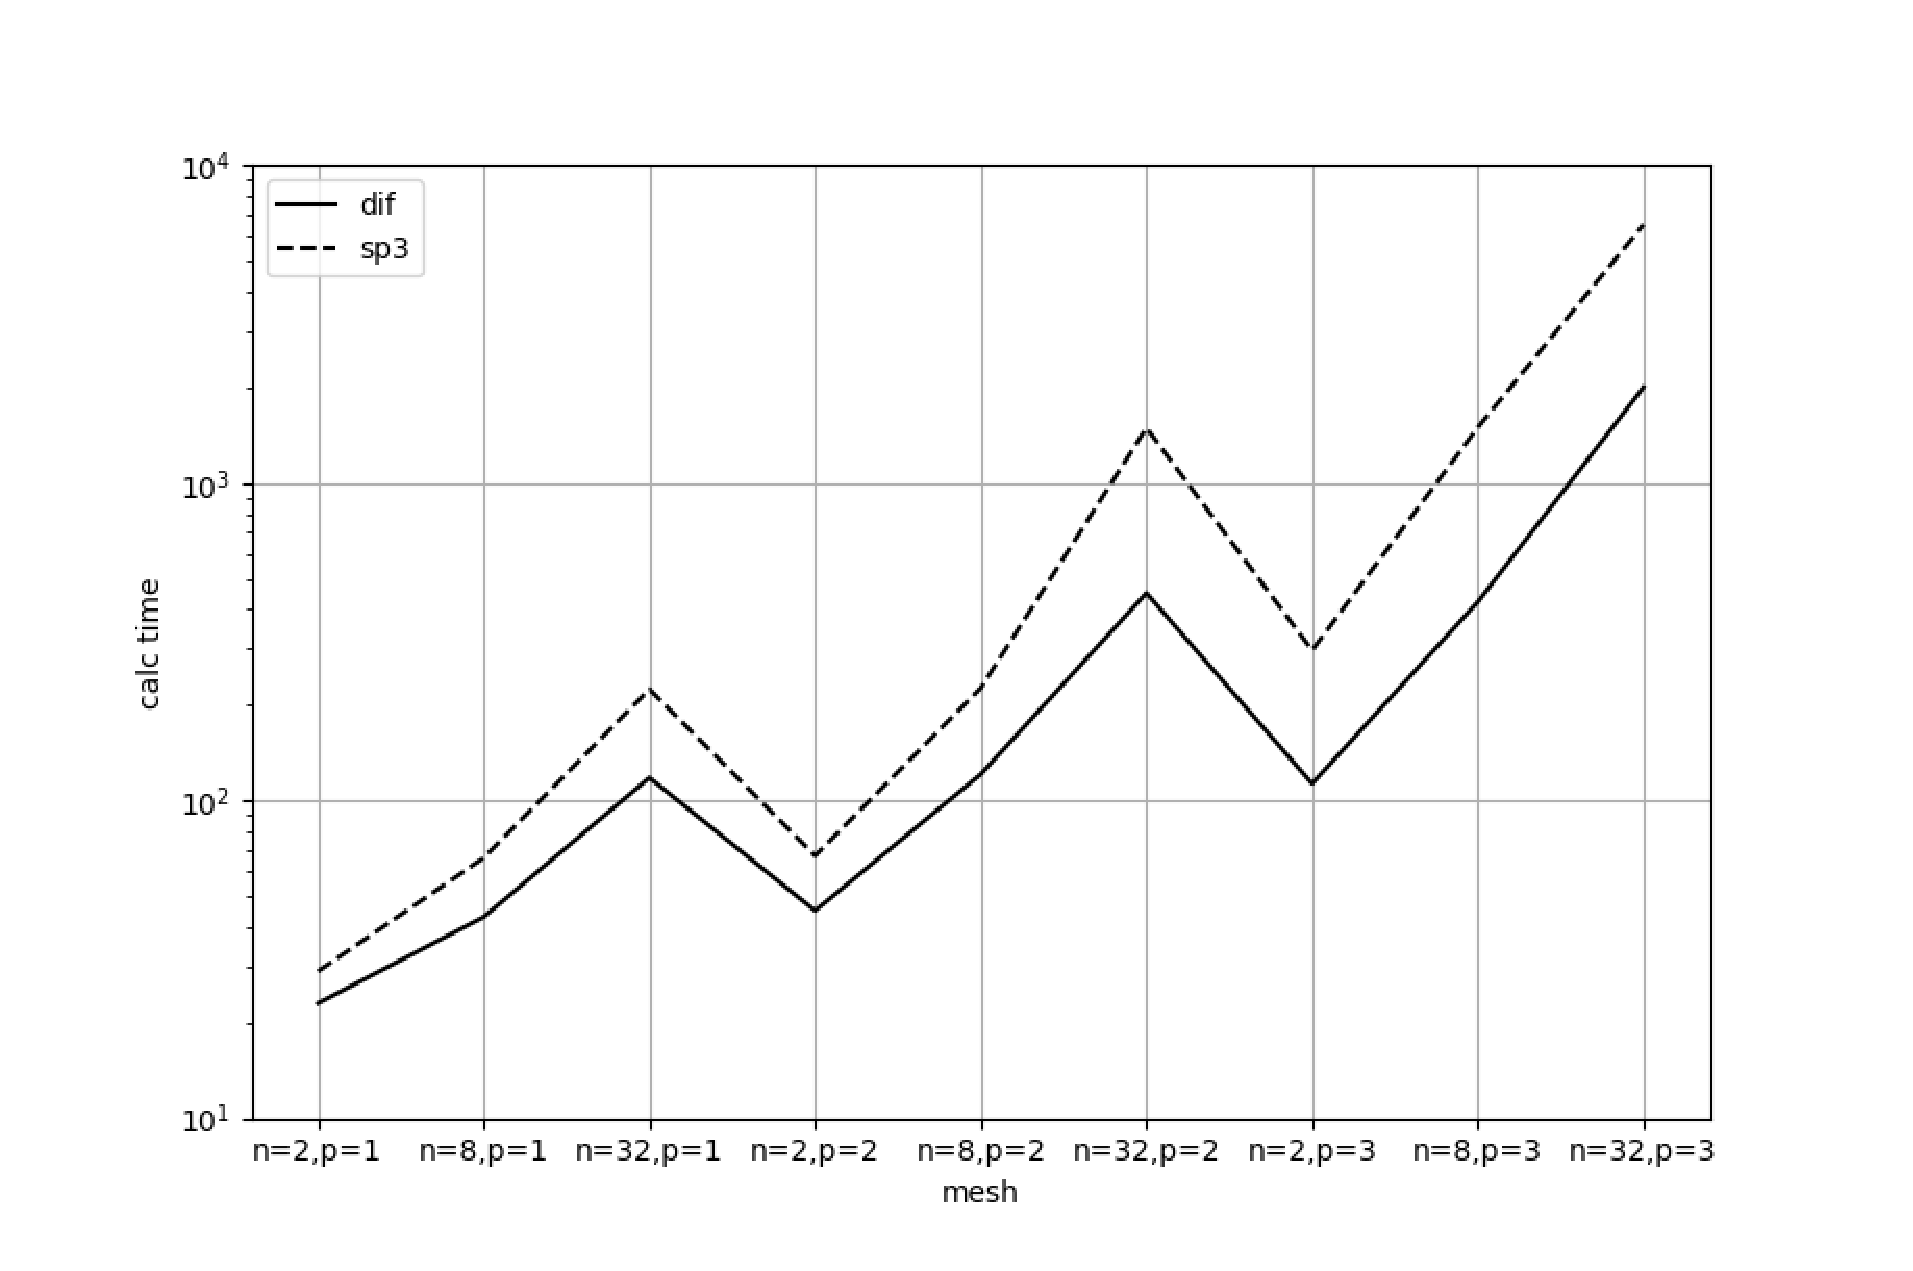
\includegraphics[width=0.7\linewidth]{calc_time.eps}
	\caption{\label{image:canonsummary} Среднее время счета динамического процесса.}
	\label{ris:calc_time}
\end{center}
\end{figure}

На рисунке \ref{ris:calc_time} показано среднее время счета диффузионных/транспортных нестационарных расчетов относительно вычислительной сетки.
Полученные данные демонстируют, что отношение времени счета между диффузионным и траспортным SP$_3$ расчетами растет при сгущении вычислительной сетки.
Например, время вычислений для SP$_3$ расчетов в среднем в 1.3 раза больше чем у диффузионных на грубой сетке ($n=2,\ p=1$), в 1.9 раза на средней сетке ($n=8,\ p=2$) и в 3.3 раза на мелкой сетке ($n=32,\ p=3$). 
В связи с этим, оптимальным вариантом сетки для траспортной SP$_3$ модели отностительно диффузионной в соотношении времени счета и точности решения для данного бэнчмарка является средняя сетка ($n=8,\ p=2$).
	
\paragraph{Заключение}

Рассмотрено численное моделирование уравнения переноса нейтронов в SP$_3$ приближении.
В качестве численного примера рассмотрен двумерный тест реактора TWIGL в трех сценариях динамического процесса.
Проводено сравнение результатов диффузионного и транспортного SP$_3$ расчетов. 
Представлены результаты исследования различных шагов по времени.
Наблюдается хорошая сходимость нестационарной задачи при уменьшении шага по времени для всех случаев.

Вычислительный алгоритм приближенного решения базируется на стандартной конечно-элементной аппроксимации по пространству при использовании лагранжевых конечных элементов.
Контроль точности решения проводился на последовательности сгущающихся сеток с использованием конечных элементов различной степени.
Матричная спектральная задача решалась с применением свободной библиотеки SLEPc.

Как и ожидалось, точность стационарных и нестационарных SP$_3$ расчетов лучше чем у диффузионных расчетов. 
С другой стороны, время вычислений для нестационарных SP$_3$ расчетов в среднем в 1.3 раза больше чем у диффузионных на грубой сетке ($n=2,\ p=1$), в 1.9 раза на средней сетке ($n=8,\ p=2$) и в 3.3 раза на мелкой сетке ($n=32,\ p=3$).

\begin{thebibliography}

\bibitem[Аввакумов и др, 2017]{avvakumov2017mm} {\it Аввакумов~А.\,В., Вабищевич~П.\,Н., Васильев~А.\,О., Стрижов~В.\,Ф.} 
Численное моделирование нестационарных задач диффузии нейтронов~// Математическое моделирование.~--- 2017.~--- Т.~29, \No~7.~--- С.~44--62.
\\
%\bibitem[Avvakumov et al, 2017]{avvakumov2017eng}
{\footnotesize{\it Avvakumov~A.\,V., Strizhov~V.\,F., Vabishchevich~P.\,N., Vasilev~A.\,O.}
Numerical modeling of neutron diffusion non-stationary problems ~// Matematicheskoe modelirovanie.~--- 2017.~--- Vol.~29, No.~7.~--- P.~44--62.}

\bibitem[Кондрушин, 2014]{kondrushin2014} {\it Кондрушин~А.\,E.} 
Развитие метода поверхностных гармоник для решения задач нейтронной пространственной кинетики в ядерных реакторах: Диссертация кандидата физико-математических наук: 05.13.18.~--- 2014.~--- 171~с.
\\
%\bibitem[Kondrushin, 2014]{kondrushin2014eng}
{\footnotesize{\it Kondrushin~A.\,E.}
Razvitie metoda poverhnostnyh garmonik dlja reshenija zadach nejtronnoj prostranstvennoj kinetiki v jadernyh reaktorah: Dissertacija kandidata fiziko-matematicheskih nauk [Development of the method of surface harmonics for solving problems of neutron spatial kinetics in nuclear reactors: PhD thesis].~--- 2014.~--- 171~p. (in Russian).\par}

\bibitem[Марчук, Лебедев, 1981]{marchuk1981} {\it Марчук~Г.\,И., Лебедев~В.\,И.} 
Численные методы в теории переноса нейтронов.~--- M.: Атомиздат.~--- 1981.~--- 455~с.
\\
%\bibitem[Marchuk, Lebedev, 1981]{marchuk1981eng}
{\footnotesize{\it Marchuk~G.\,I., Lebedev~V.\,I.}
Chislennye metody v teorii perenosa nejtronov [Numerical methods in the theory of neutron transport].~--- M.: Atomizdat.~--- 1981.~--- 455~p. (in Russian).\par}
    
\bibitem[Avvakumov et al, 2017]{avvakumov2017} {\it Avvakumov~A.\,V., Strizhov~V.\,F., Vabishchevich~P.\,N., Vasilev~A.\,O.} Spectral properties of dynamic processes in a nuclear reactor ~// Annals of Nuclear Energy.~--- 2017.~--- Vol.~99.~--- P.~68--79.

\bibitem[Avvakumov et al, 2018]{avvakumov2018} {\it Avvakumov~A.\,V., Strizhov~V.\,F., Vabishchevich~P.\,N., Vasilev~A.\,O.} State change modal method for numerical simulation of dynamic processes in a nuclear reactor ~// Progress in Nuclear Energy.~--- 2018.~--- Vol.~106.~--- P.~240--261.

\bibitem[Azmy, Sartori, 2010]{azmy2010} {\it Azmy~Y, Sartori~E.} Nuclear Computational Science: A Century in Review~--- Springer Science \& Business Media, 2010.~--- 470~p.

\bibitem[Beckert, Grundmann, 2008]{beckert2008} {\it Beckert~C., Grundmann~U.}Development and verification of a nodal approach for solving the multigroup SP3 equations~// Annals of Nuclear Energy.~--- 2008.~--- Vol.~35, No.~1.~--- P.~75--86.

\bibitem[Bell, Glasstone, 1970]{bell1970} {\it Bell~G.\,I., Glasstone~S.} Nuclear reactor theory~--- US Atomic Energy Commission, Washington, DC (United States), 1970.

\bibitem[Brewster, 2018]{brewster2018} {\it Brewster~W.\,J.} Development and Monte Carlo validation of a finite element reactor analysis framework~--- Missouri University of Science and Technology, 2018.

\bibitem[Brantley, Larsen, 2000]{brantley2000} {\it Brantley~P.\,S., Larsen~E.\,W.} The simplified P3 approximation~// Nuclear science and engineering.~--- 2000.~--- Vol.~134, No.~1.~--- P.~1--21.

\bibitem[Carreno et al, 2017]{carreno2017} {\it Carreno~A., Vidal-Ferrandiz~A., Verdu~G., Ginestar~D.} The eigenvalue problem Alpha, lambda and gamma modes and its applications~// Proceedings of 2017 international congress on advances in nuclear power plants (ICAPP2017).~--- P.~2573.

\bibitem[Joo et al, 2004]{joo2004} {\it Joo~H.\,G., Cho~J.\,Y., Kim~K.\,S., Lee~C.\,C., Zee~S.\,Q.} Methods and performance of a three-dimensional whole-core transport code DeCART~--- In:Physor, 2004.

\bibitem[Downar et al, 2009]{downar2009} {\it Downar~T., Xu~Y., Seker~V., Hudson~N.} Theory manual for the PARCS kinetics core simulator module~--- Department of Nuclear Engineering and Radiological Sciences University of Michigan, 2009.

%\bibitem[Evans, 1990]{evans1990} {\it Evans~L.\,C.} Weak convergence methods for nonlinear partial differential equations~---  American Mathematical Soc., 1990.~--- No.~74.

\bibitem[Gelbard, 1961]{gelbard1961} {\it Gelbard~E.\,M.} Simplified spherical harmonics equations and their use in shielding problems~--- Westinghouse Electric Corp. Bettis Atomic Power Lab., 1961.

%\bibitem[Habetler, Martino, 1961]{habetler1961} {\it Habetler~G.\,J., Martino~M.\,A.} Existence theorems and spectral theory for the multigroup diffusion model~--- Proc. of the Eleventh Symposium in Applied Mathematics of the American Mathematical Society, 1961.~--- Vol.~11.

\bibitem[Hageman, Yasinsky, 1969]{hageman1969} {\it Hageman~L.\,A., Yasinsky~J.\,B.} Comparison of alternating-direction time-differencing methods with other implicit methods for the solution of the neutron group-diffusion equations~// Nuclear Science and Engineering.~--- 1969.~--- Vol.~38, No.~1.~--- P.~8--32.

\bibitem[Lawrence, 1986]{lawrence1986} {\it Lawrence~R.\,D.} Progress in nodal methods for the solution of the neutron diffusion and transport equations~// Progress in Nuclear Energy.~--- 1986.~--- Vol.~17, No.~3.~--- P.~271--301.

\bibitem[Lewis, Miller, 1984]{lewis1984} {\it Lewis~E.\,E., Miller~W.\,F.} Computational methods of neutron transport~--- John Wiley and Sons, 1984.~--- 401~p.

\bibitem[Logg et al, 2012]{logg2012} {\it Logg~A., Mardal~K.\,E., Wells~G.} Automated solution of differential equations by the finite element method: The FEniCS book~--- Springer Science \& Business Media, 2012.~--- Vol.~84.~--- 401~p.

\bibitem[McClarren, 2010]{mcclarren2010} {\it McClarren~R.\,G.} Theoretical aspects of the simplified Pn equations~// Transport Theory and Statistical Physics.~--- 2010.~--- Vol.~39, No.~2--4.~--- P.~73--109.

\bibitem[Quarteroni, Valli, 2008]{quarteroni2008} {\it Quarteroni~A., Valli~A.} Numerical approximation of partial differential equations~--- Weinheim: Springer Science \& Business Media, 2008.~--- Vol.~23.

\bibitem[Sutton, Aviles, 1996]{sutton1996} {\it Sutton~T.\,M., Aviles~B.\,N.} Diffusion theory methods for spatial kinetics calculations~// /Progress in nuclear energy.~--- 1996.~--- Vol.~30, No.~2.~--- P.~119--182.

\bibitem[Stacey, 2007]{stacey2007} {\it Stacey~W.\,B.} Nuclear Reactor Physics~--- Weinheim: wiley-vch, 2007.~--- 735~p.

\bibitem[Tada et al, 2008]{tada2008} {\it Tada~K., Yamamoto~A., Yamane~Y., Kitamuray~Y.} Applicability of the diffusion and simplified P3 theories for pin-by-pin geometry of BWR~// Journal of nuclear science and technology.~--- 2008.~--- Vol.~45, No.~10.~--- P.~997--1008.

\bibitem[Verdu et al, 2010]{verdu2010} {\it Verdu~G., Ginestar~D., Roman~J., Vidal~V.} 3D alpha modes of a nuclear power reactor~// Journal of nuclear science and technology.~--- 2010.~--- Vol.~47, No.~5.~--- P.~501--514.


\end{thebibliography}

\end{document}
